% 西北农林科技大学科技类及IT类课程论文文档类(LaTeX模板)
\documentclass{nwafucoursepaper}

% 载入需要的宏包
% % =========浮动体增强宏包=========
% \usepackage{floatrow}
% \floatsetup[figure]{objectset=centering, margins=centering}

% % ========处理标题的宏包=========
% \usepackage[labelsep=quad]{caption}
% \usepackage{varioref}
% \usepackage{subfig}

% =========引号宏包=========
\usepackage{csquotes}

%%% Local Variables:
%%% mode: latex
%%% TeX-master:"../main.tex"
%%% End:

% 进行必要的设置
% ====================================================================================
% cquotes宏包的中文引号样式
% ====================================================================================
\DeclareQuoteStyle{zhquotestyle}% style name
    {\symbol{"201C}}% opening outer mark
    {\symbol{"201D}}% closing outer mark
    {\symbol{"2018}}% opening inner mark
    {\symbol{"2019}}% closing inner mark

\setquotestyle{zhquotestyle}

% ====================================================================================
% 改变表格字体
% ====================================================================================
\BeforeBeginEnvironment{tabular}{\small}%

%%% Local Variables:
%%% mode: latex
%%% TeX-master:"../main.tex"
%%% End:

% 专用术语宏命令进行必要的设置
% ====================================================================================
% 西北农林科技大学各单位名称
% ====================================================================================
\newcommand{\nwafu}{西北农林科技大学}
\newcommand{\cie}{信息工程学院}

% ============自定义专有名词命令============
\newcommand{\cl}{\texttt{C}语言}
\newcommand{\ccpp}{\texttt{C/C++}}
\newcommand{\win}{\texttt{Windows}}
\newcommand{\ide}{\texttt{IDE}}
\newcommand{\gcc}{\texttt{GCC}}
\newcommand{\gpp}{\texttt{G++}}
\newcommand{\gnu}{\texttt{GNU}}
\newcommand{\cb}{\texttt{Code::Blocks}}
\newcommand{\mgww}{\texttt{MinGW}}
\newcommand{\mgw}{\texttt{MinGW32}}
\newcommand{\mgwww}{\texttt{MinGW-w64}}
\newcommand{\lumos}{\texttt{Linux}、\texttt{Unix}、\texttt{Mac OS}}
\newcommand{\unix}{\texttt{UNIX}}
\newcommand{\lnx}{\texttt{Linux}}
\newcommand{\mk}{\texttt{make}}
\newcommand{\ph}{\texttt{Path}}
\newcommand{\cmdd}{\texttt{cmd}}
\newcommand{\gdb}{\texttt{gdb}调试器}
\newcommand{\vside}{\texttt{Visual Studio}}
\newcommand{\mfile}{\texttt{Makefile}}
\newcommand{\tgt}{\texttt{target}}
\newcommand{\prqt}{\texttt{prerequisites}}
\newcommand{\cbv}{\texttt{17.12}}
\newcommand{\db}{\texttt{DEBUG}}
\newcommand{\dbger}{\texttt{Debugger}}
\newcommand{\cdb}{\texttt{cdb}调试器}
\newcommand{\gdbcmd}{\texttt{(gdb)}}
\newcommand{\bug}{\texttt{BUG}}
\newcommand{\ieee}{\texttt{IEEE754}标准}
\newcommand{\ascii}{\texttt{ASCII}}
\newcommand\vararg{变长形参列表}
\newcommand\varargfun{\vararg{}函数}
\newcommand{\cg}{\texttt{CGraph2D} 图形库}
\newcommand{\git}{分布式版本控制系统\texttt{Git}}
\newcommand{\github}{\texttt{Github}平台}
% ====================================


%%% Local Variables:
%%% mode: latex
%%% TeX-master:"../main.tex"
%%% End:

% % % 用于排版LaTeX代码并同时输出结果的环境定义(若无此需要,可以不加载)
% % \usepackage{tcolorbox}
\usepackage{accsupp}  % PDF accessibility support

\tcbuselibrary{skins, minted, xparse}

% make line numbers unable to be selected
% ref: https://liam.page/2013/11/04/LaTeX-listings-copy/
\ExplSyntaxOn
\newcommand\emptyaccsupp[1]{
  \BeginAccSupp{ActualText={}} #1 \EndAccSupp{}
}

\renewcommand\theFancyVerbLine{
  \emptyaccsupp{
    \textcolor[rgb]{0.5, 0.5, 1.0}{
      \scriptsize\arabic{FancyVerbLine}
    }
  }
}
\ExplSyntaxOff

\makeatletter
\tcbset{
  % see tcbminted.code.tex, def of "minted options"
  % minted options/.store in=\kvtcb@minted@options,
  minted options app/.code=\appto\kvtcb@minted@options{,#1}
}
\makeatother

% define new option
\tcbset{
  example options/.style={
    skin=bicolor,
    colbacklower=white,
    fonttitle=\sffamily,
    minted options app={
      % line numbers
      linenos,
      numberfirstline=true,
      stepnumber=2,
      numbersep=5pt,
      % break point
      breakbefore=\\,
    }
  },
  example title/.style 2 args={
    title=Example\ifblank{#1}{}{ #1}\ifblank{#2}{}{: #2}
  }
}


% new env: example
% #1 - <kv list>, tcb-listing options
% #2 - <token list>, title
\makeatletter
\NewTCBListing[auto counter]{example}{ O{} m }{
  example options,
  example title={\thetcbcounter}{#2},
  #1
}
\makeatother

% new env: example*
% like example, except that it is un-numbered
\NewTCBListing{example*}{ O{} m }{
  example options,
  example title={}{#2},
  #1
}

% % % 用于排版LaTeX命令代码的环境定义(若无此需要,可以不加载)
% % \RequirePackage{tcolorbox}
\tcbuselibrary{documentation}

\ExplSyntaxOn
\makeatletter

% #1 = tcb options
% #2 = clist of 3-tuple, "{name}{arg}{desc}, {}{}{}, ..."
\NewDocumentEnvironment{docCommands}{ O{} m }
  {
    \tcbset{#1}
    \begin{tcb@manual@entry}
    \tcb_doc_heads:n {#2}
    \nobreak\tcbset{before~ upper=}
    \kvtcb@doc@body@command@before
    \ignorespaces
  }
  {
    \ifvmode\else\unskip\fi
    \kvtcb@doc@body@command@after
    \end{tcb@manual@entry}
  }

% to use \seq_pop_right:NN
\seq_new:N \l_tcb_heads_seq

% #1 = clist of 3-tuple, "{csname}{arg}{desc}, {}{}{}, ..."
\cs_new:Nn \tcb_doc_heads:n
  {
    \seq_set_from_clist:Nn \l_tcb_heads_seq {#1}
    \seq_pop_left:NN \l_tcb_heads_seq \l_tmpa_tl
    \exp_after:wN \tcb_doc_head:nnnn \l_tmpa_tl 
      {after~ skip=0pt, enlarge~ bottom~ by=0pt}
    \seq_pop_right:NN \l_tcb_heads_seq \l_tmpa_tl
    \seq_map_inline:Nn \l_tcb_heads_seq
      {
        \tcb_doc_head:nnnn ##1 
          {before~ skip=0pt, after~ skip=0pt, enlarge~ bottom~ by=0pt}
      }
    \exp_after:wN \tcb_doc_head:nnnn \l_tmpa_tl 
      {before~ skip=0pt, enlarge~ bottom~ by=-0.2\baselineskip}
  }

% #1 = command csname
% #2 = arg spec
% #3 = command description
% #4 = tcb options
\cs_new:Nn \tcb_doc_head:nnnn
  {
    \begin{tcb@doc@head}{doc@head@command, #4}
    \strut
    \tcb@Print@Com{#1}\tcb@index@Com{#1}
    \protected@edef\@currentlabel{\noexpand\tcb@cs{#1}}\label{com:#1}
    {\ttfamily #2}
    \gdef\kvtcb@doc@description{#3}%  result of \tcbset{doc description=#3}
    \tcb@doc@do@description
    \end{tcb@doc@head}
  }

\makeatother
\ExplSyntaxOff

\endinput

% usage
\begin{docCommands}
{
  {menu}
    {\oarg{input sep}\marg{menu sequence}}
    {\oarg{input sep} defaults to |>|},
  {directory}
    {\oarg{input sep}\marg{menu sequence}}
    {\oarg{input sep} defaults to |/|},
  {keys}
    {\oarg{input sep}\marg{menu sequence}}
    {\oarg{input sep} defaults to |+|}
}
  content
\end{docCommands}

%% ----------------------------
%% begin: original definitions
%%   from tcbdocumentation.code.tex
%%   link https://github.com/T-F-S/tcolorbox/blob/master/tex/latex/tcolorbox/tcbdocumentation.code.tex
%% ----------------------------

%\newenvironment{docCommand}[3][]{\tcbset{#1}%
%  \begin{tcb@manual@entry}%
%  \begin{tcb@doc@head}{doc@head@command}%
%  \tcb@Print@Com{#2}\tcb@index@Com{#2}\protected@edef\@currentlabel{\noexpand\tcb@cs{#2}}\label{com:#2}{\ttfamily #3}%
%  \tcb@doc@do@description%
%  \end{tcb@doc@head}\nobreak\tcbset{before upper=}\kvtcb@doc@body@command@before\ignorespaces}%
%  {\ifvmode\else\unskip\fi\kvtcb@doc@body@command@after\end{tcb@manual@entry}}
%
%\newenvironment{tcb@manual@entry}{\begin{list}{}{%
%  \setlength{\leftmargin}{\kvtcb@doc@left}%
%  \setlength{\itemindent}{0pt}%
%  \setlength{\itemsep}{0pt}%
%  \setlength{\parsep}{0pt}%
%  \setlength{\rightmargin}{\kvtcb@doc@right}%
%  }\item}{\end{list}}
%
%\newtcolorbox{tcb@doc@head}[1]{blank,colback=white,colframe=white,
%  code={\tcbdimto\tcb@temp@grow@left{-\kvtcb@doc@indentleft}%
%        \tcbdimto\tcb@temp@grow@right{-\kvtcb@doc@indentright}},
%  grow to left by=\tcb@temp@grow@left,%
%  grow to right by=\tcb@temp@grow@right,
%  sidebyside,sidebyside align=top,
%  sidebyside gap=-\tcb@w@upper@real,
%  phantom=\phantomsection,%
%  enlarge bottom by=-0.2\baselineskip,#1}

%% ----------------------------
%% end: original definitions
%% ----------------------------

% 乱数假文宏包
\usepackage{zhlipsum}
\usepackage{hyperref}
\usepackage{listings}
\lstset{
  numbers=left,
  stepnumber=1,
  showspaces=false,
  showtabs=false,
  breaklines=true,
  showstringspaces=false,
  breakatwhitespace=true,
  commentstyle=\color{green},
  keywordstyle=\color{blue},
  stringstyle=\color{red},
  basicstyle=\ttfamily,
  moredelim=[il][\textcolor{pgrey}]{$$},
  moredelim=[is][\textcolor{pgrey}]{\%\%}{\%\%}
}

\title{\bfseries\sffamily E-Exercise学习答题网站使用说明书}
\author{\zihao{4} \fangsong 封钰震(1951362)\\\fangsong 信息管理与信息系统 \\\small \songti 管理科学与工程系}
\date{\small \today}

% 摘要内容
\begin{abstract}
\end{abstract}
% 关键词内容(用英文","分割)
\keywords{}

%biblatex宏包的参考文献数据源加载方式
\addbibresource[location=local]{bib/example.bib}
\begin{document} %在document环境中撰写文档
% 排版标题
\maketitle
\thispagestyle{empty}
% 排版摘要
% \makeabstract

\section{前言}

本网站可以通过IP地址进行访问,登录界面的URL为\url{http://47.103.73.100:8081/ExerciseOnline/user/toLogin}。在答辩完成后本网站所有源代码将在GitHub上进行开源,遵循MIT License开源协议,网址为\url{https://github.com/Feng-Yz/Java-Homework/tree/main/FinalProject/Exercise-Web-Online}。

\section{运行环境}

经测试,该网站可以在如下运行环境中运行:
\begin{itemize}
  \item Oracle JDK 14.0.2或OpenJDK 11.0.12(其他版本未进行测试)
  \item MySQL 5.7.34
\end{itemize}

\section{附件说明}

在提交的大作业文件夹中,包括:
\begin{enumerate}
  \item \verb|eExercise|文件夹,其中是项目文件;
  \item \verb|ExerciseOnline-0.0.1-SNAPSHOT.jar|JAR包;
  \item \verb|eExercise.sql|SQL文件,其中包括新建表单、插入数据的SQL语句;
  \item \verb|eExercise_trigger.sql|SQL文件,其中包括新建触发器的SQL语句;
  \item 包含使用说明书的PDF文件;
  \item 包含大作业报告的PDF文件。
\end{enumerate}

在\verb|eExercise|文件夹中,包括:
\begin{enumerate}
  \item Maven的\verb|pom.xml|文件;
  \item \verb|src|文件夹,其中\verb|main|文件夹中为本项目的主要内容,\verb|test|文件夹中为测试代码(无需使用)。
\end{enumerate}

\verb|main|文件夹中\verb|java/com/Yuzhen/ExerciseOnline/|的内容具体如下:
\begin{itemize}
    \item \verb|auxiliary/|:辅助类,主要包括一些辅助函数,例如:对知识和习题模板的处理、对上传文件重命名等;
    \item \verb|entity/|:数据库实体类;
    \item \verb|controller/|:控制器类,用于处理Http请求、配置URL映射等;
    \item \verb|service/|:用于处理业务逻辑;
    \item \verb|repository/|:用于数据访问的接口;
    \item \verb|NoLoginException.java|:用于处理未登录异常;
    \item \verb|GlobalExceptionHandleController.java|:用于处理其他异常;
    \item \verb|ExerciseOnlineApplication.java|:主类。
\end{itemize}

\verb|main|文件夹中\verb|resources/|的内容具体如下:
\begin{itemize}
    \item \verb|application.properties|:应用程序的配置文件;
    \item \verb|mappers/|:Mybatis的XML映射文件;
    \item \verb|static/|:网页静态资源;
    \item \verb|templates/|:网页模板。
\end{itemize}

\section{部署说明}

\subsection{方式一:直接通过JAR包运行}

首先将JAR包放入Tomcat对应的文件夹中,再进入该文件夹中通过\verb|java|命令运行JAR包(此时可使用\verb|nohup|不挂断地运行),例如:
\begin{lstlisting}
  scp -r ExerciseOnline-0.0.1-SNAPSHOT.jar root@47.103.73.100:/root/apache-tomcat-8.5.41/ExerciseOnline/
  nohup java -jar ExerciseOnline-0.0.1-SNAPSHOT.jar &
\end{lstlisting}

该方式下使用的数据库为作者的云端数据库。部署完成后,使用URL\url{http://[IP]:8081/ExerciseOnline/user/toLogin}即可访问。\textbf{注意,一定要在Tomcat上配置8081端口(Tomcat的默认端口号为8080);同时若将其部署在服务器上,要配置服务器安全组}。若想将端口号设为8080,则需在应用程序的配置文件\verb|application.properties|中作如下更改:
\begin{lstlisting}
  server.port=8080
\end{lstlisting}

建议直接访问作者部署完成的网站:\url{http://47.103.73.100:8081/ExerciseOnline/user/toLogin}。

\subsection{方式二:通过IDEA运行}

IDEA已经集成了Maven,不需要再下载Maven。使用IDEA打开该项目,第一步,使用Maven下载相关资源;第二步,待下载完毕后再右击\verb|ExerciseOnlineApplication.java|主类,点击\verb|Run|。如图\ref{idea_instruct}所示。
\begin{figure}[h]
  \centering
  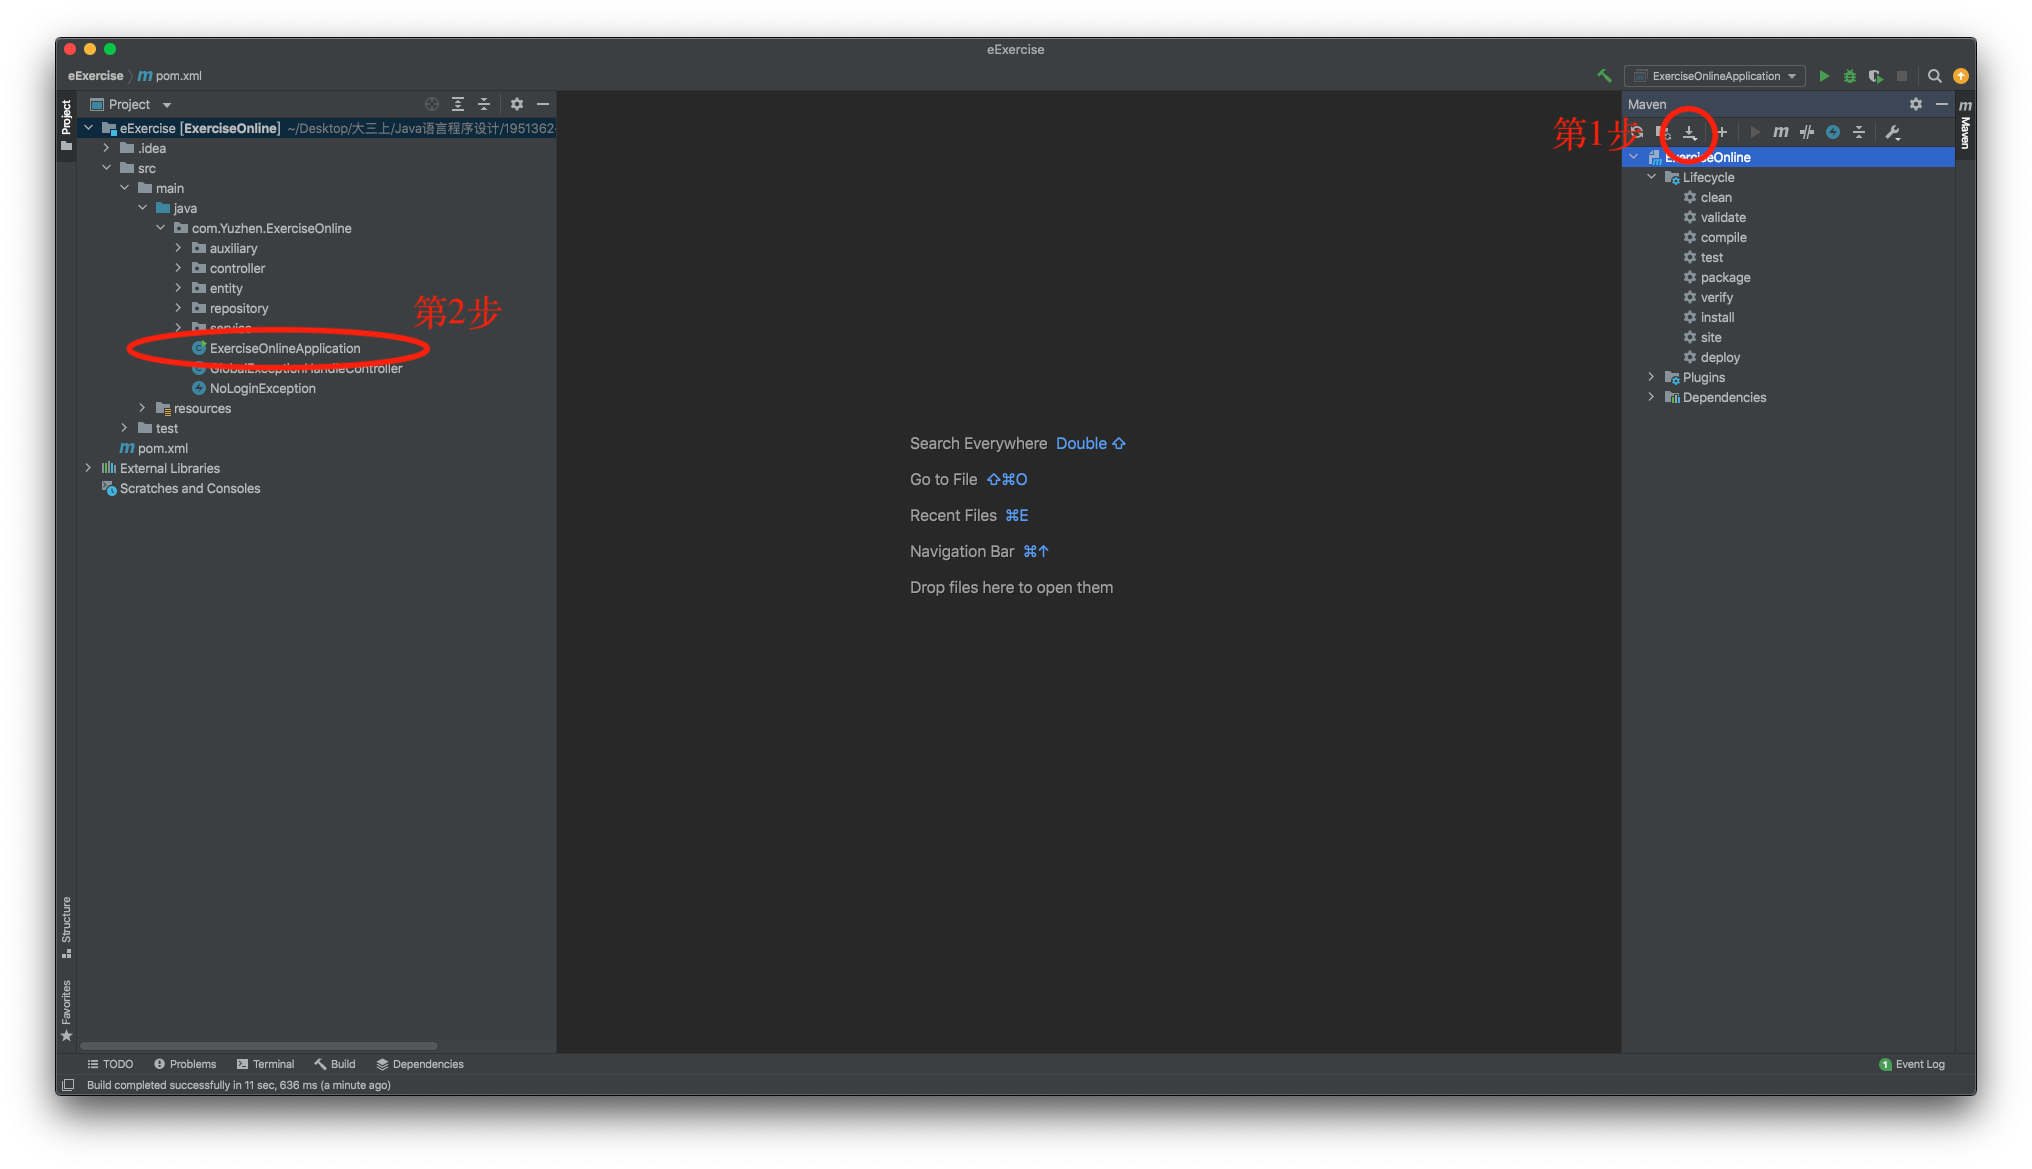
\includegraphics[width=0.8\textwidth]{idea_instruct.png}
  \caption{通过IDEA运行}
  \label{idea_instruct}
\end{figure}

该方式下使用的数据库仍为作者的云端数据库。

\subsection{方式三:使用本地数据库}

新建数据库,运行\verb|eExercise.sql|与\verb|eExercise_trigger.sql|两个SQL文件,再在应用程序的配置文件\verb|application.properties|中作如下更改:
\begin{lstlisting}
  spring.datasource.url=jdbc:mysql://[IP or localhost]:3306/[Table name]?characterEncoding=utf8&autoReconnect=true&useSSL=false
  spring.datasource.username=[Database username]
  spring.datasource.password=[Database user password]
\end{lstlisting}

\newpage

\section{功能说明}

\subsection{基本功能}

\begin{figure}[htp]
  \centering
  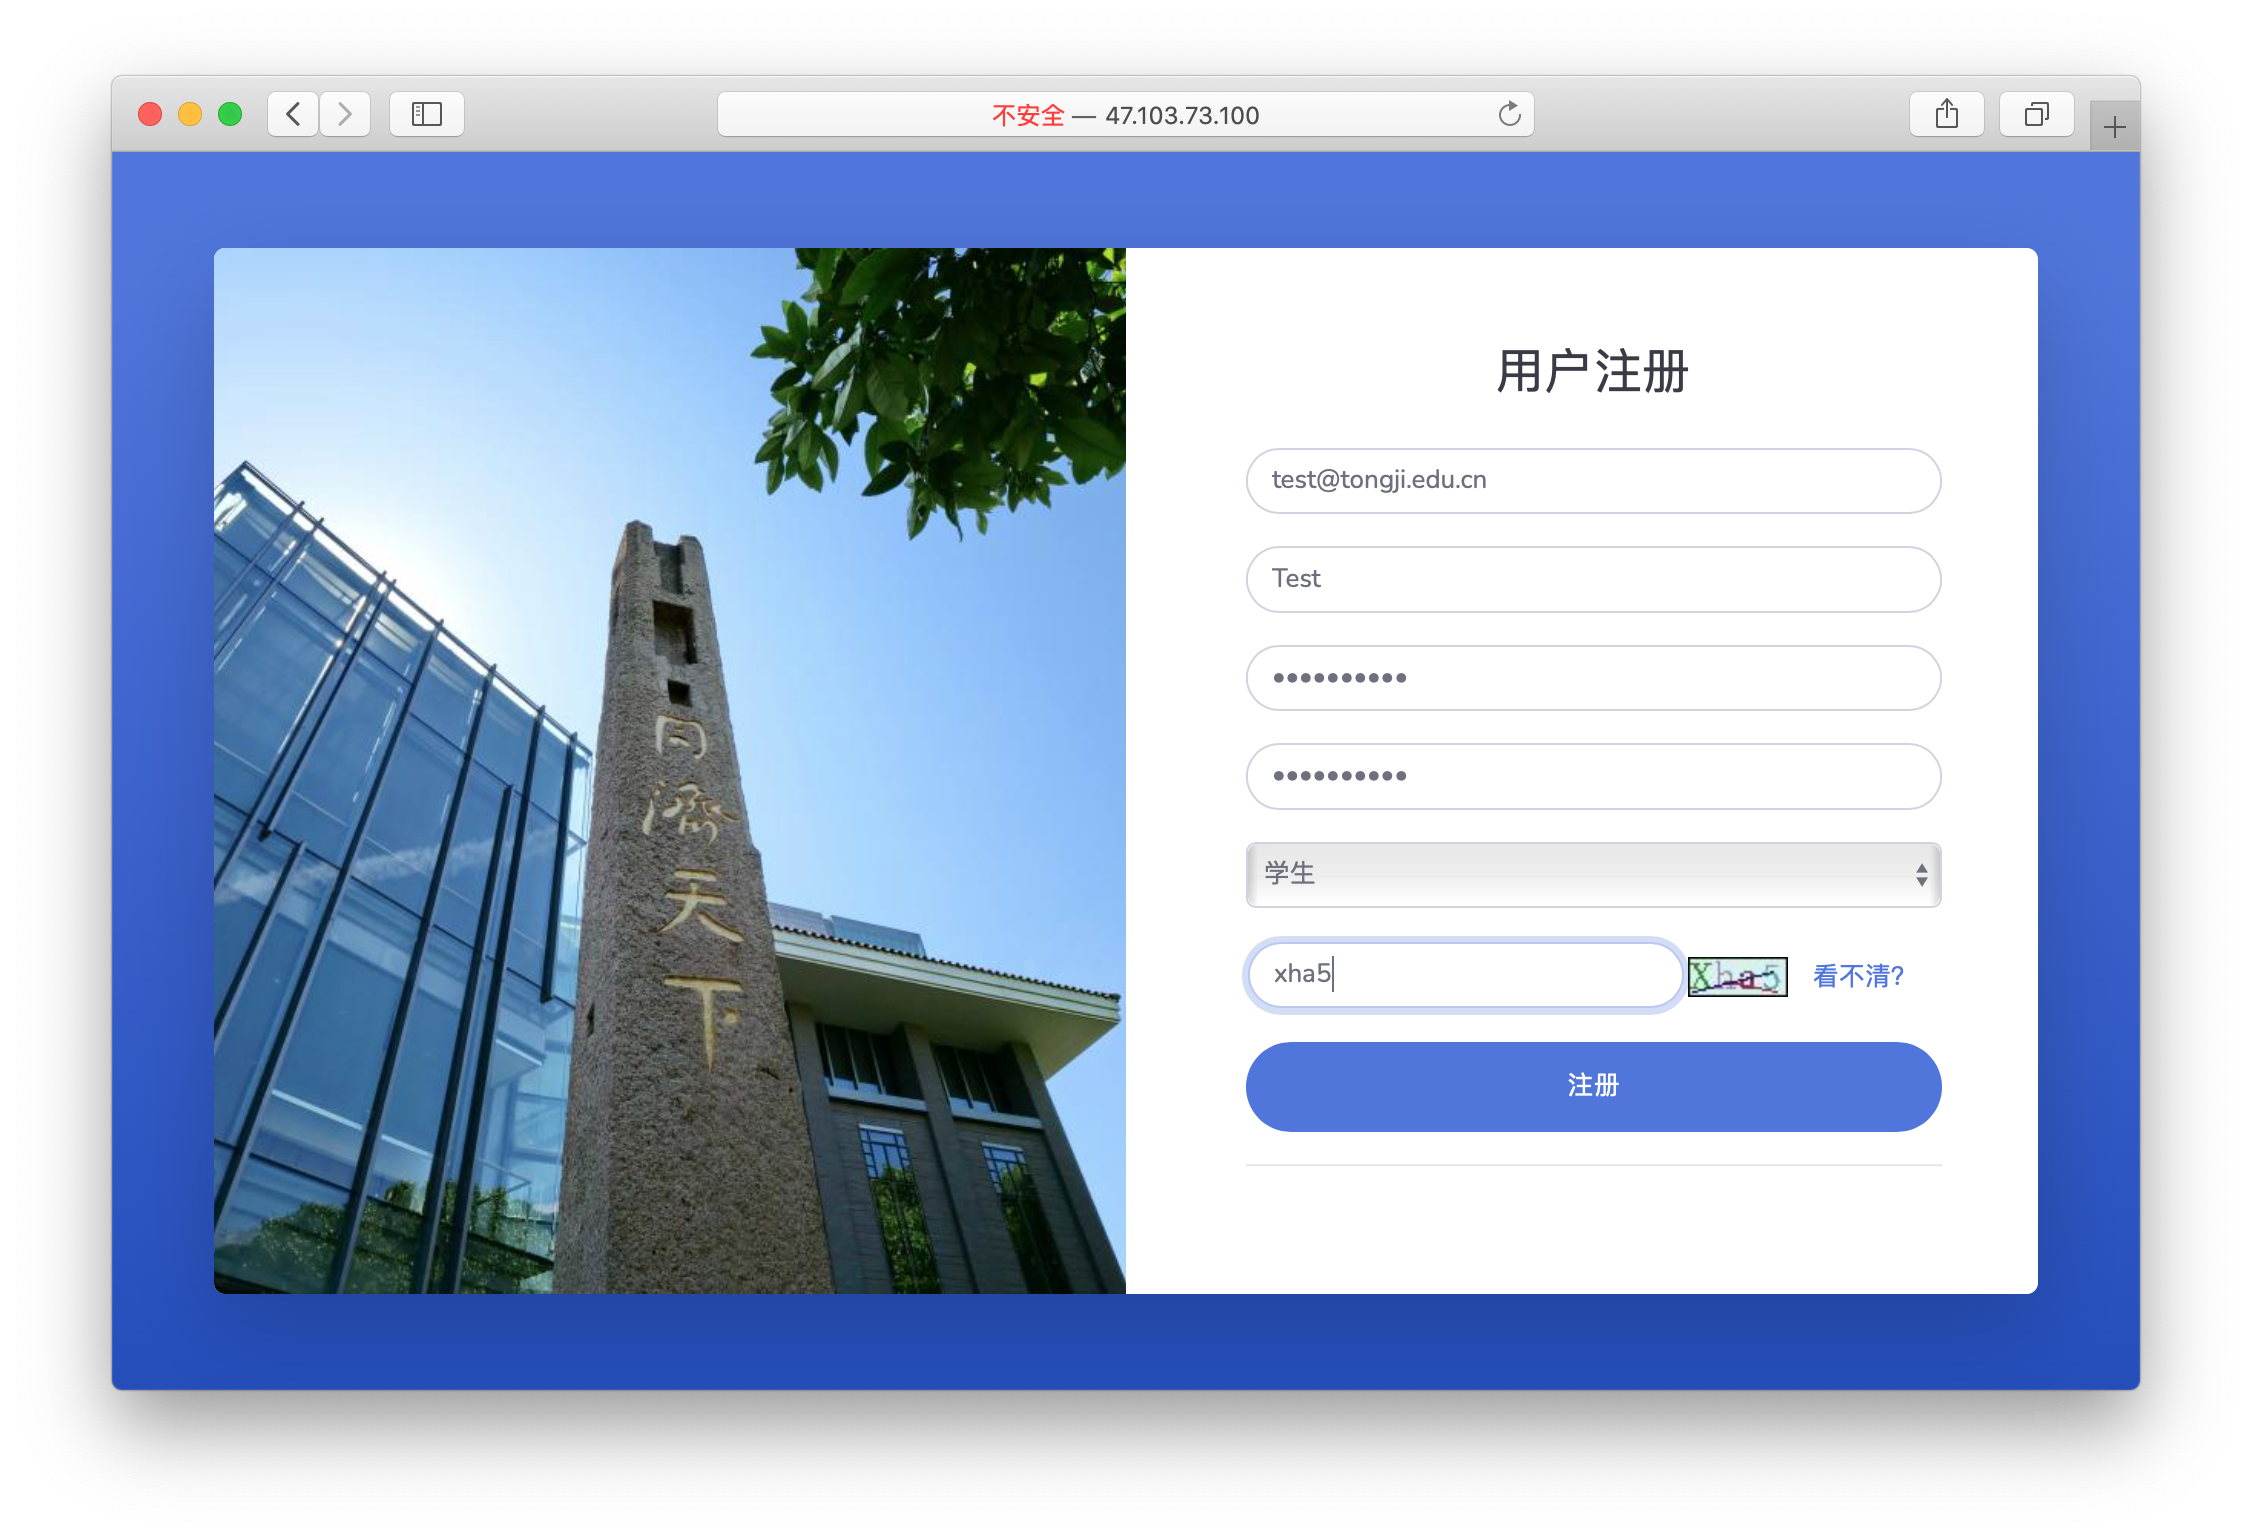
\includegraphics[width=0.8\textwidth]{register.png}
  \caption{注册页面}
  \label{register}
\end{figure}

\begin{figure}[htp]
  \centering
  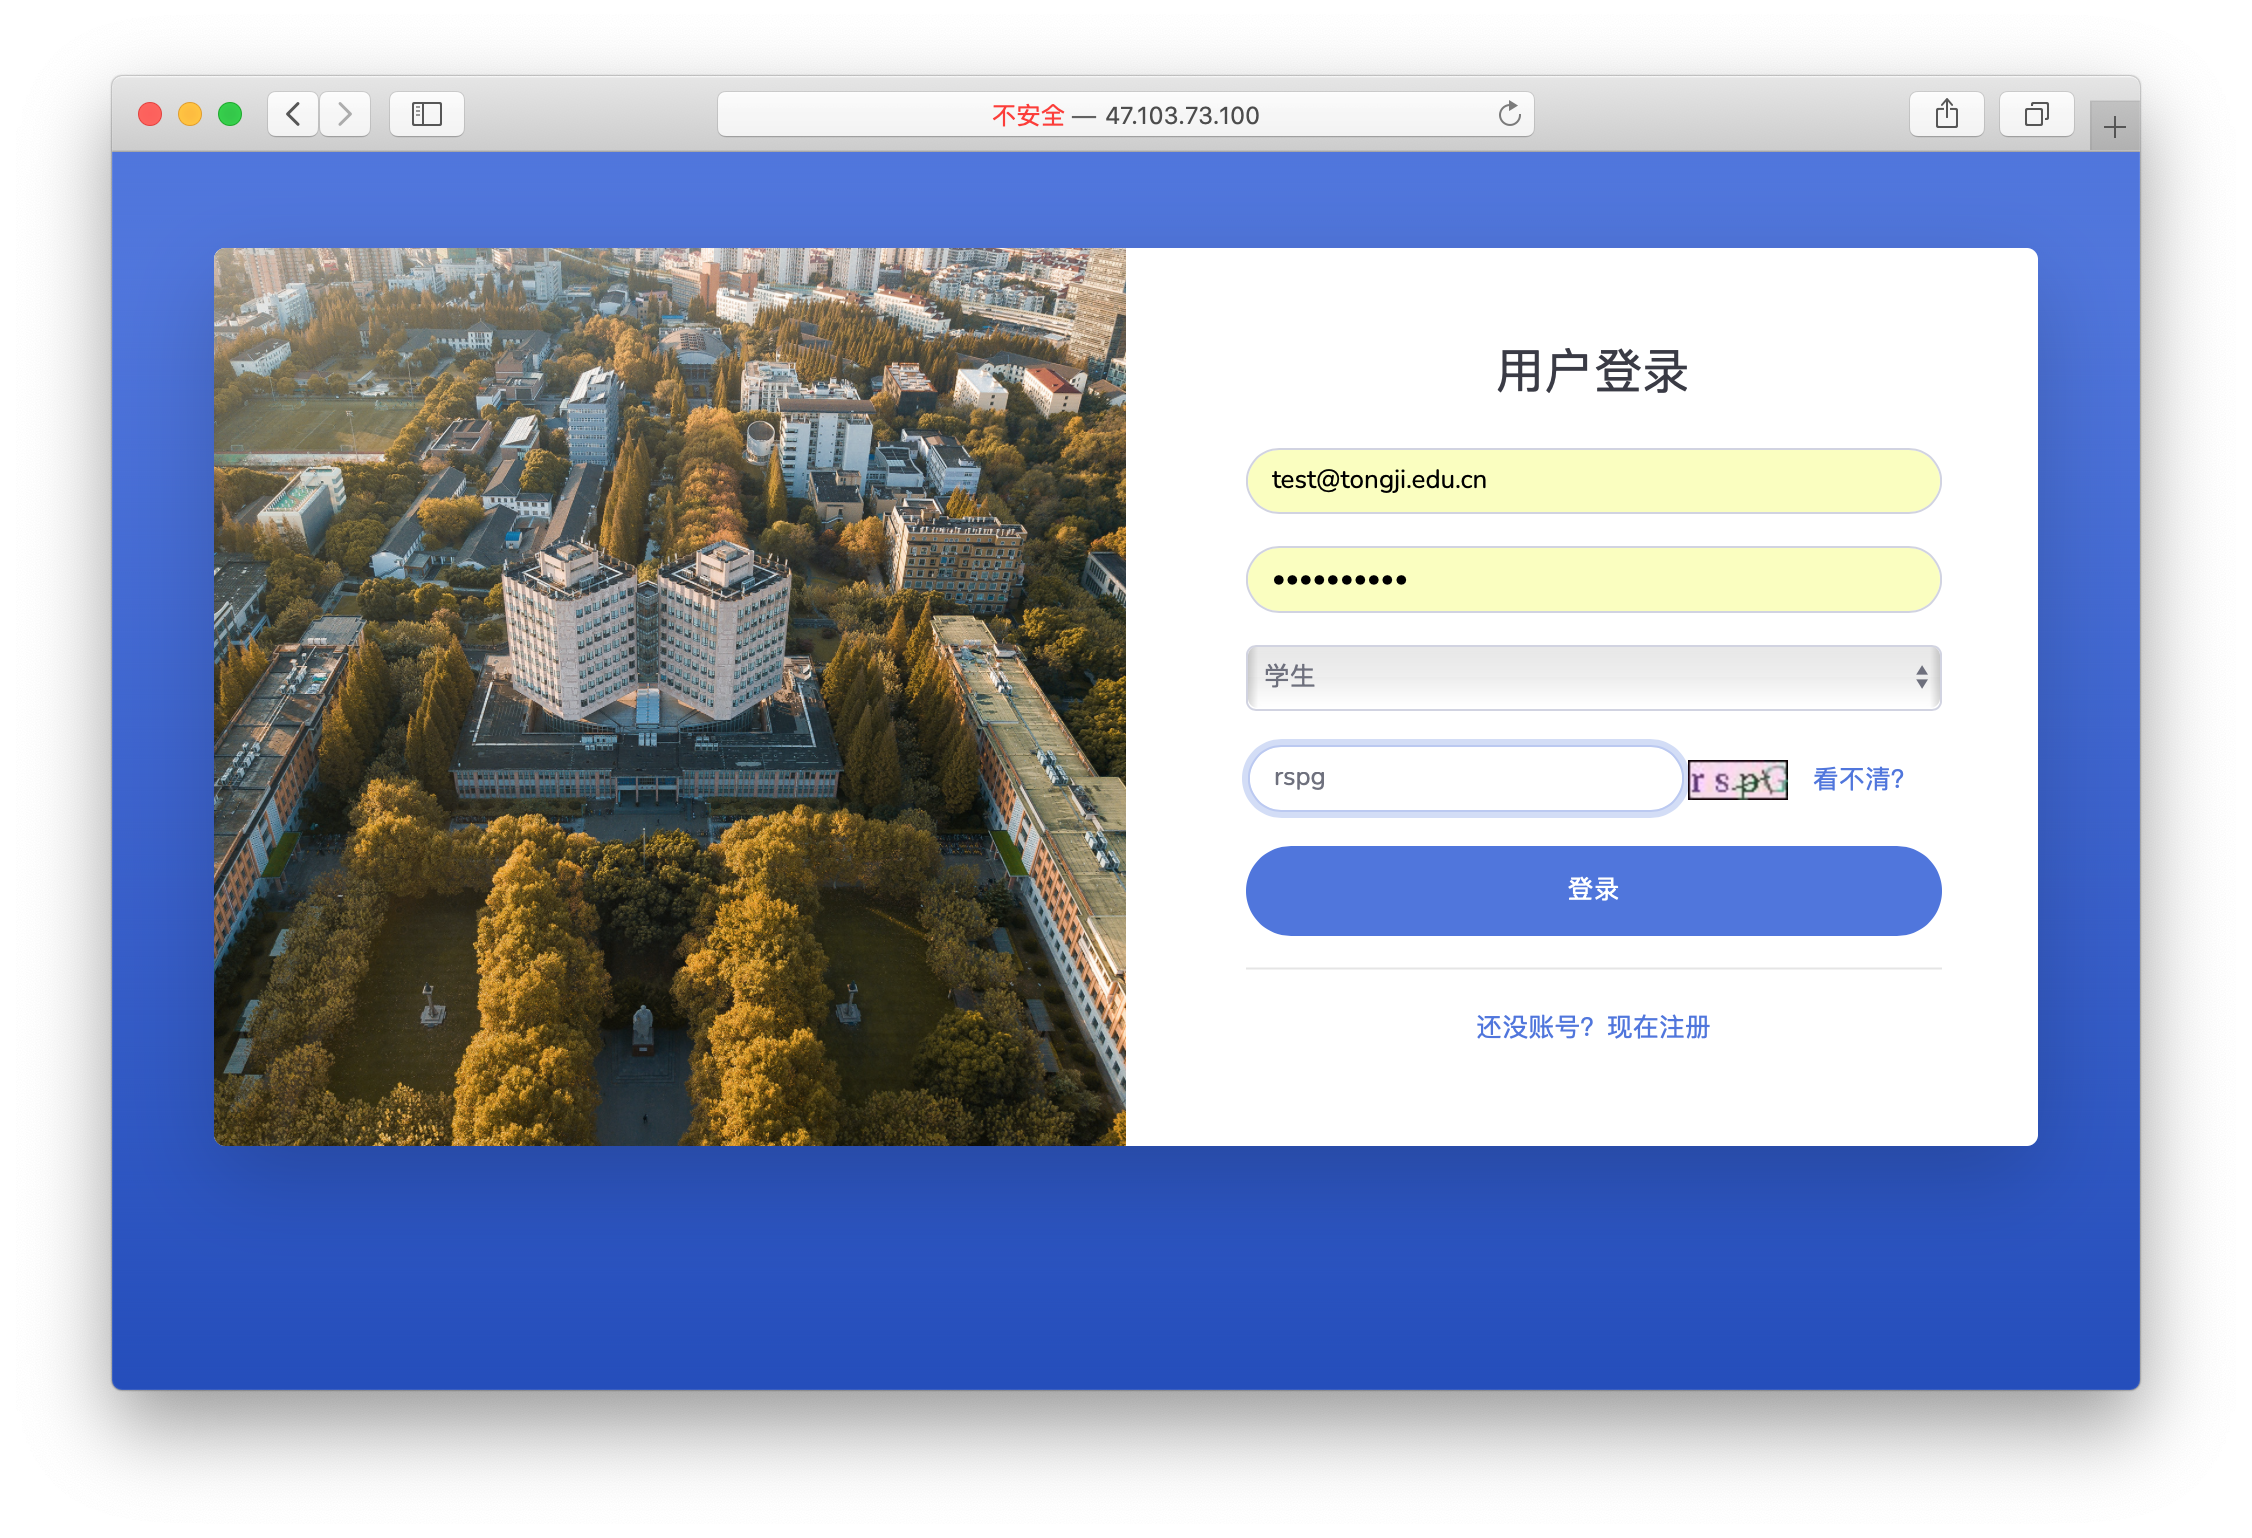
\includegraphics[width=0.8\textwidth]{login.png}
  \caption{登录页面}
  \label{login}
\end{figure}

网站的基本功能包括用户注册、用户登录,另有验证码防止恶意行为。目前,网站并不允许用户自行注册为管理员与教师,只能注册为学生。注册时,系统会查看邮箱是否已经被注册。若已经被注册,则向前端返回警报。

注册完成后,现在您可以通过邮箱\verb|test@tongji.edu.cn|和密码\verb|test123456|进行访问了!注册和登录界面分别如图\ref{register}和\ref{login}所示。

\subsection{知识功能}

\begin{figure}[htp]
  \centering
  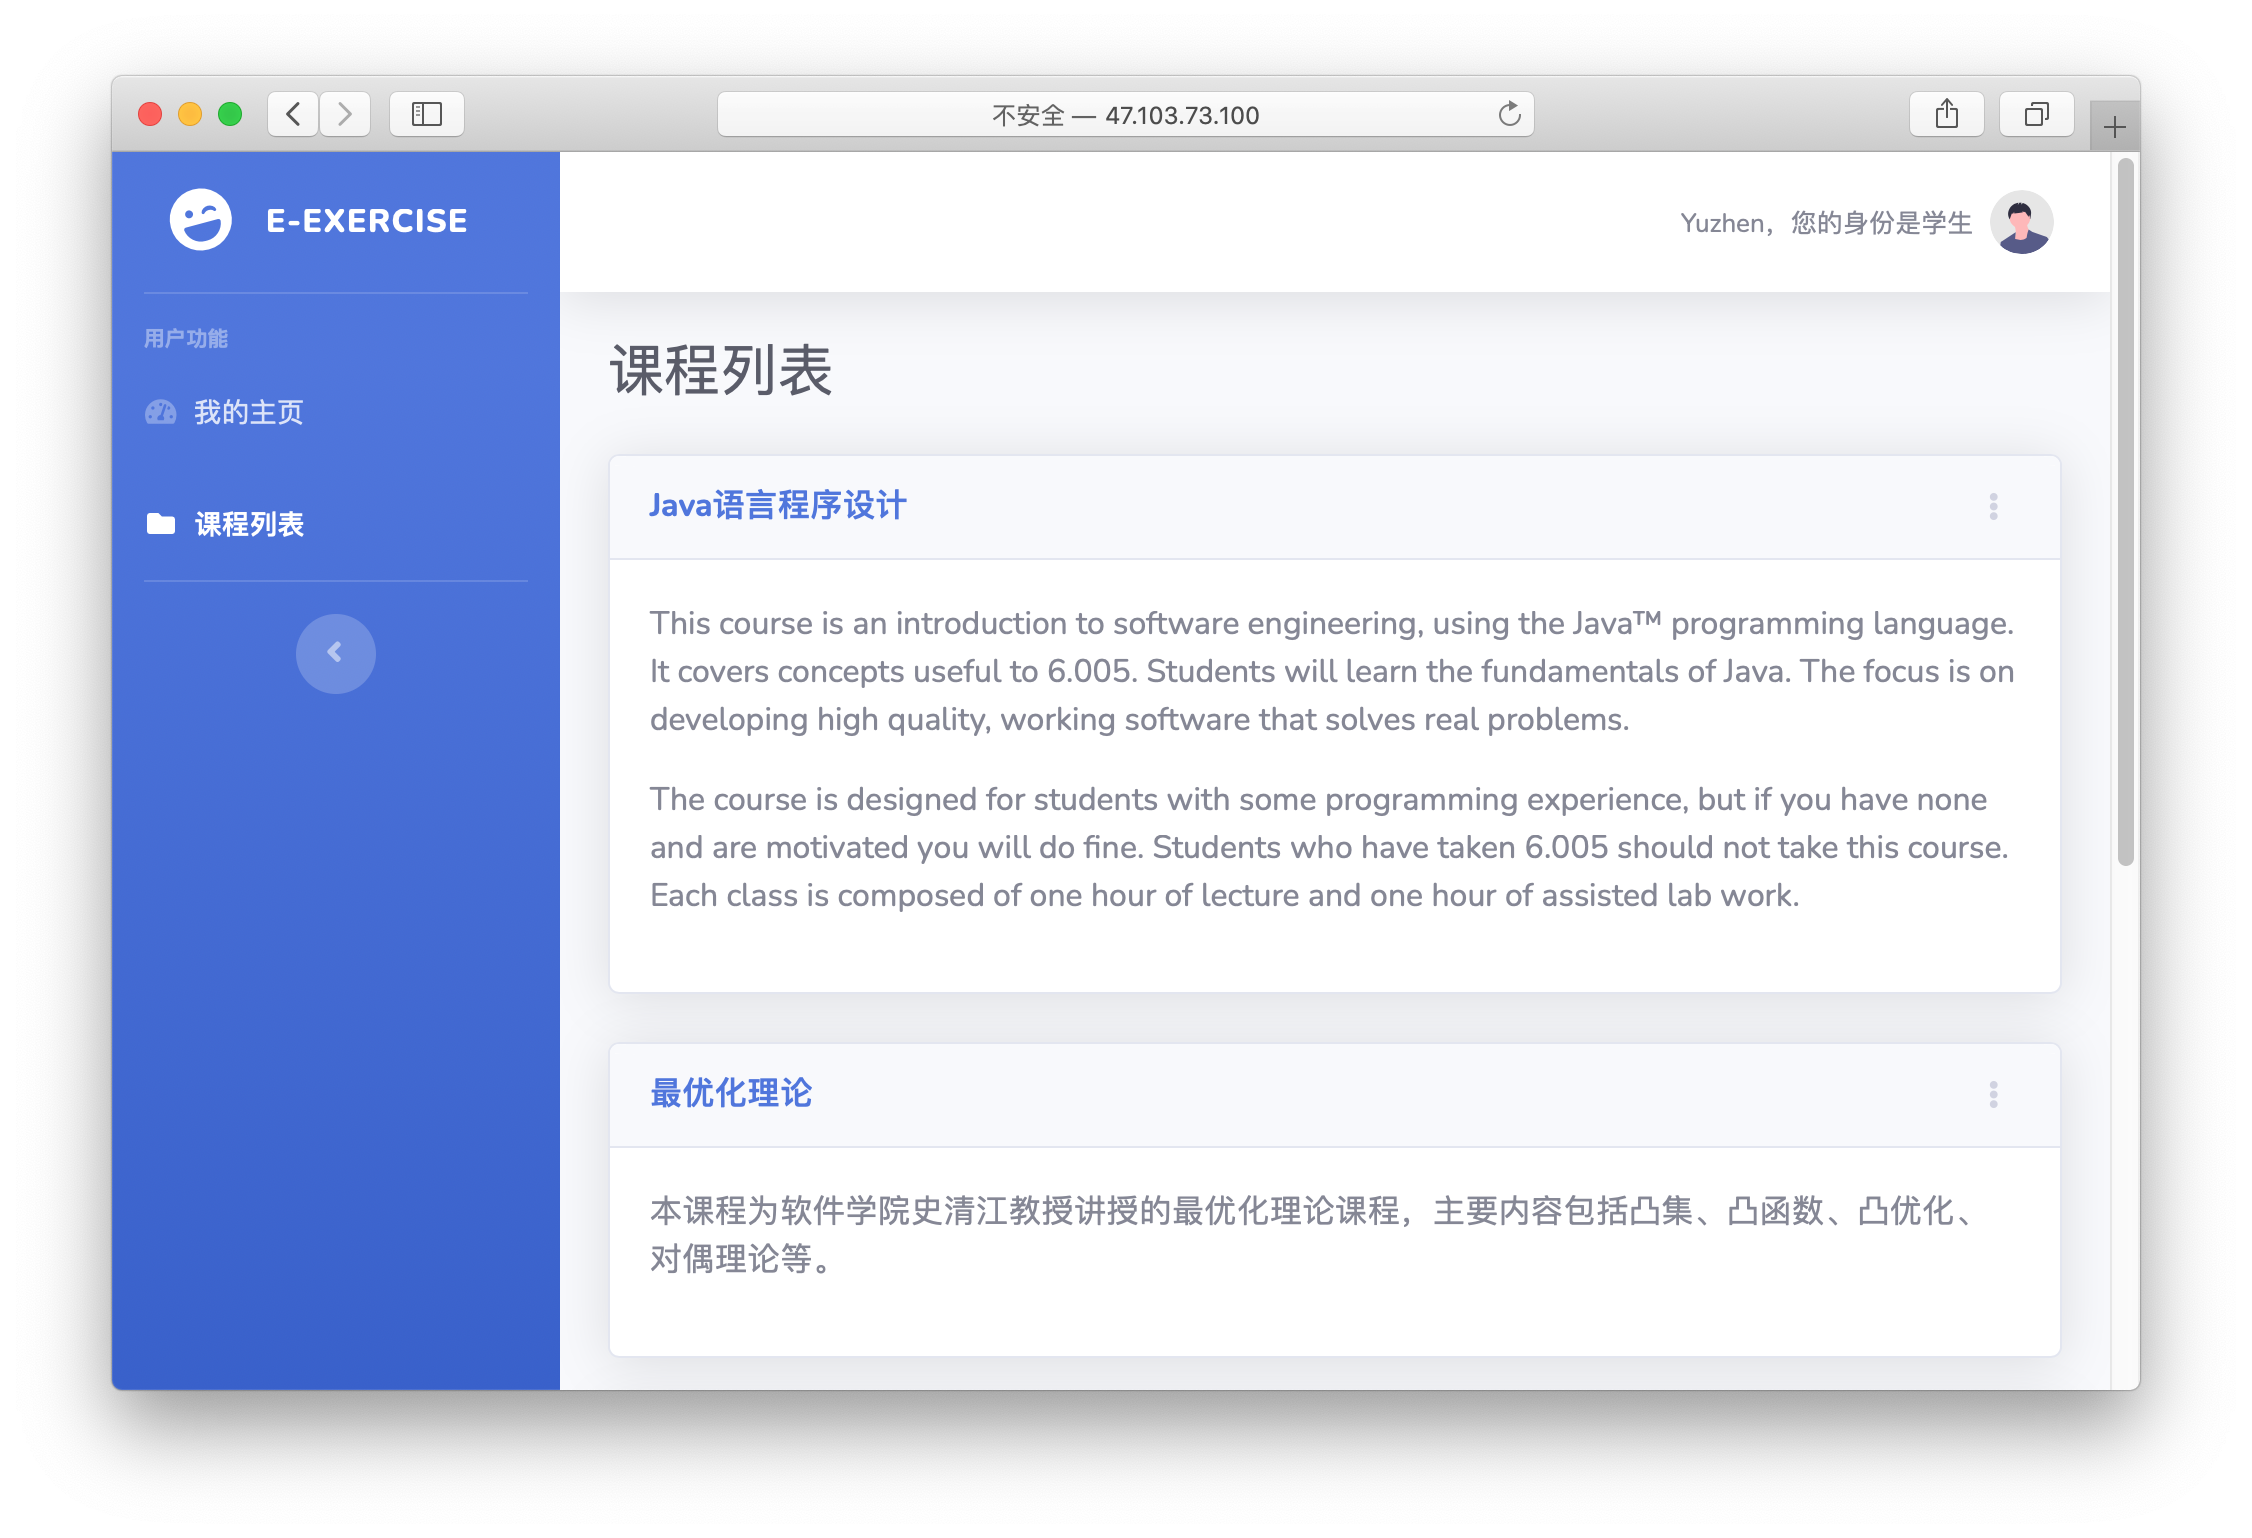
\includegraphics[width=0.8\textwidth]{subject_list.png}
  \caption{课程列表}
  \label{subject_list}
\end{figure}

\begin{figure}[htp]
  \centering
  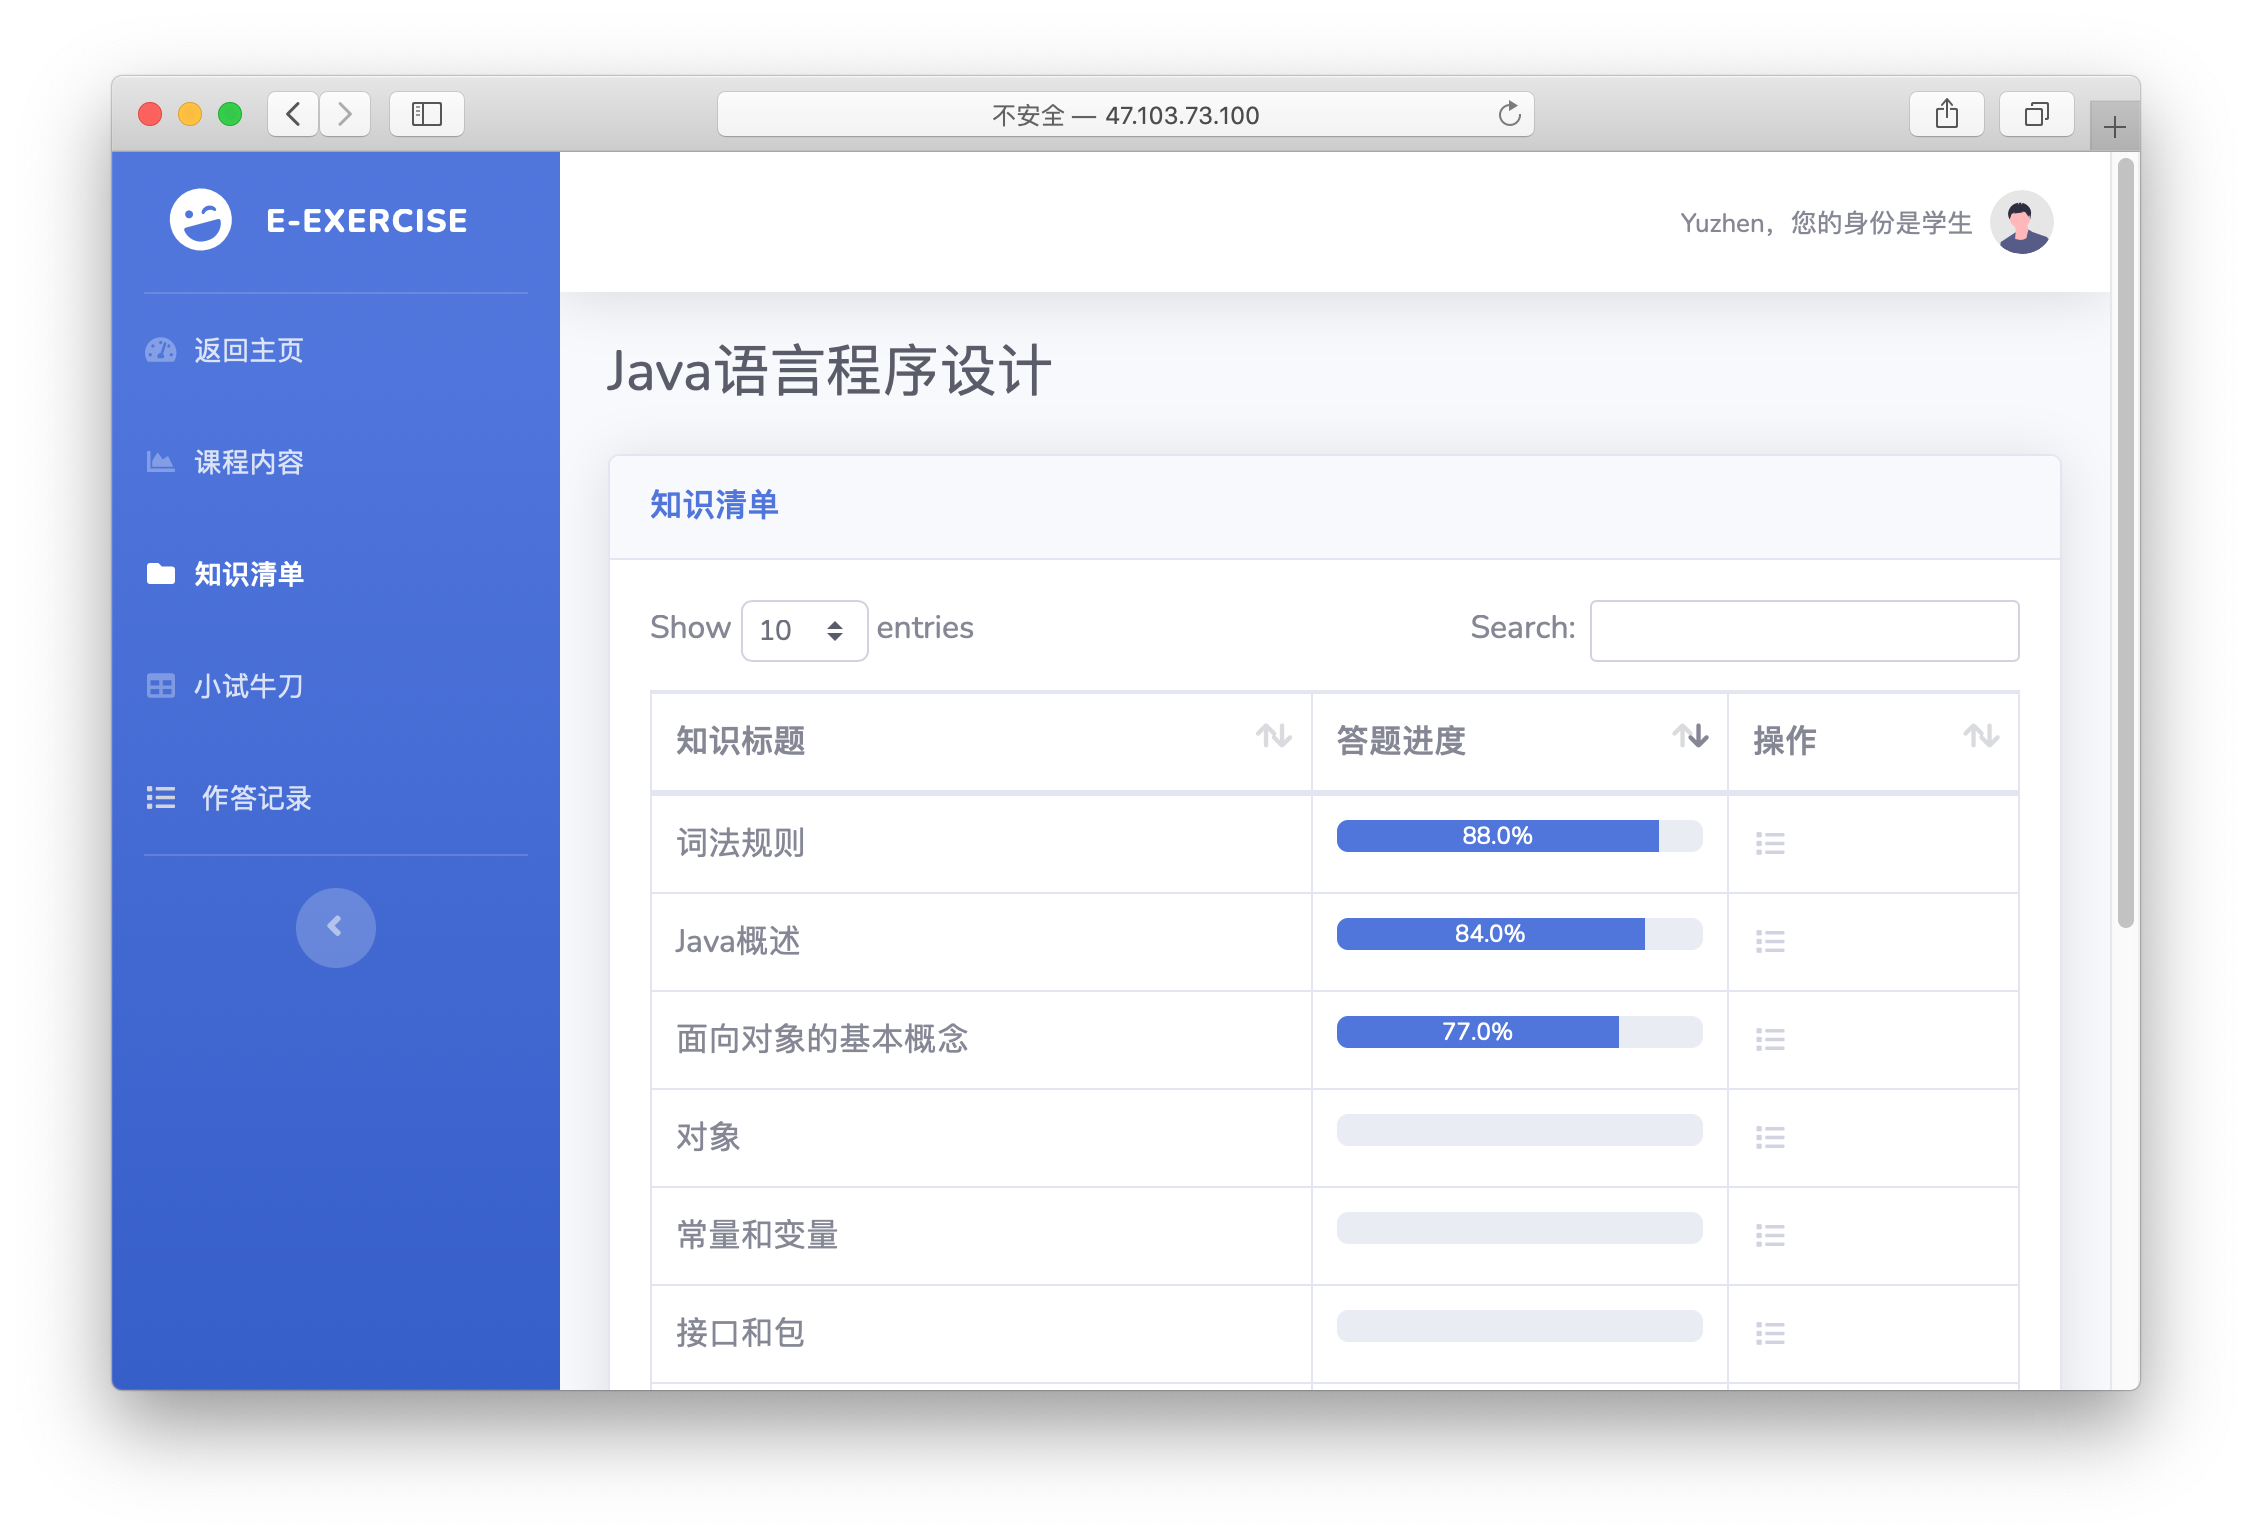
\includegraphics[width=0.8\textwidth]{knowledge_list.png}
  \caption{知识清单}
  \label{knowledge_list}
\end{figure}

对于学生用户来说,可以查看课程列表,进入课程页面后可以查看知识清单和具体知识内容,主页和知识清单页面都有学习进度的显示(主要依据答题情况)。课程列表、知识清单两界面分别如图\ref{subject_list}和\ref{knowledge_list}所示。

\begin{figure}[htp]
  \centering
  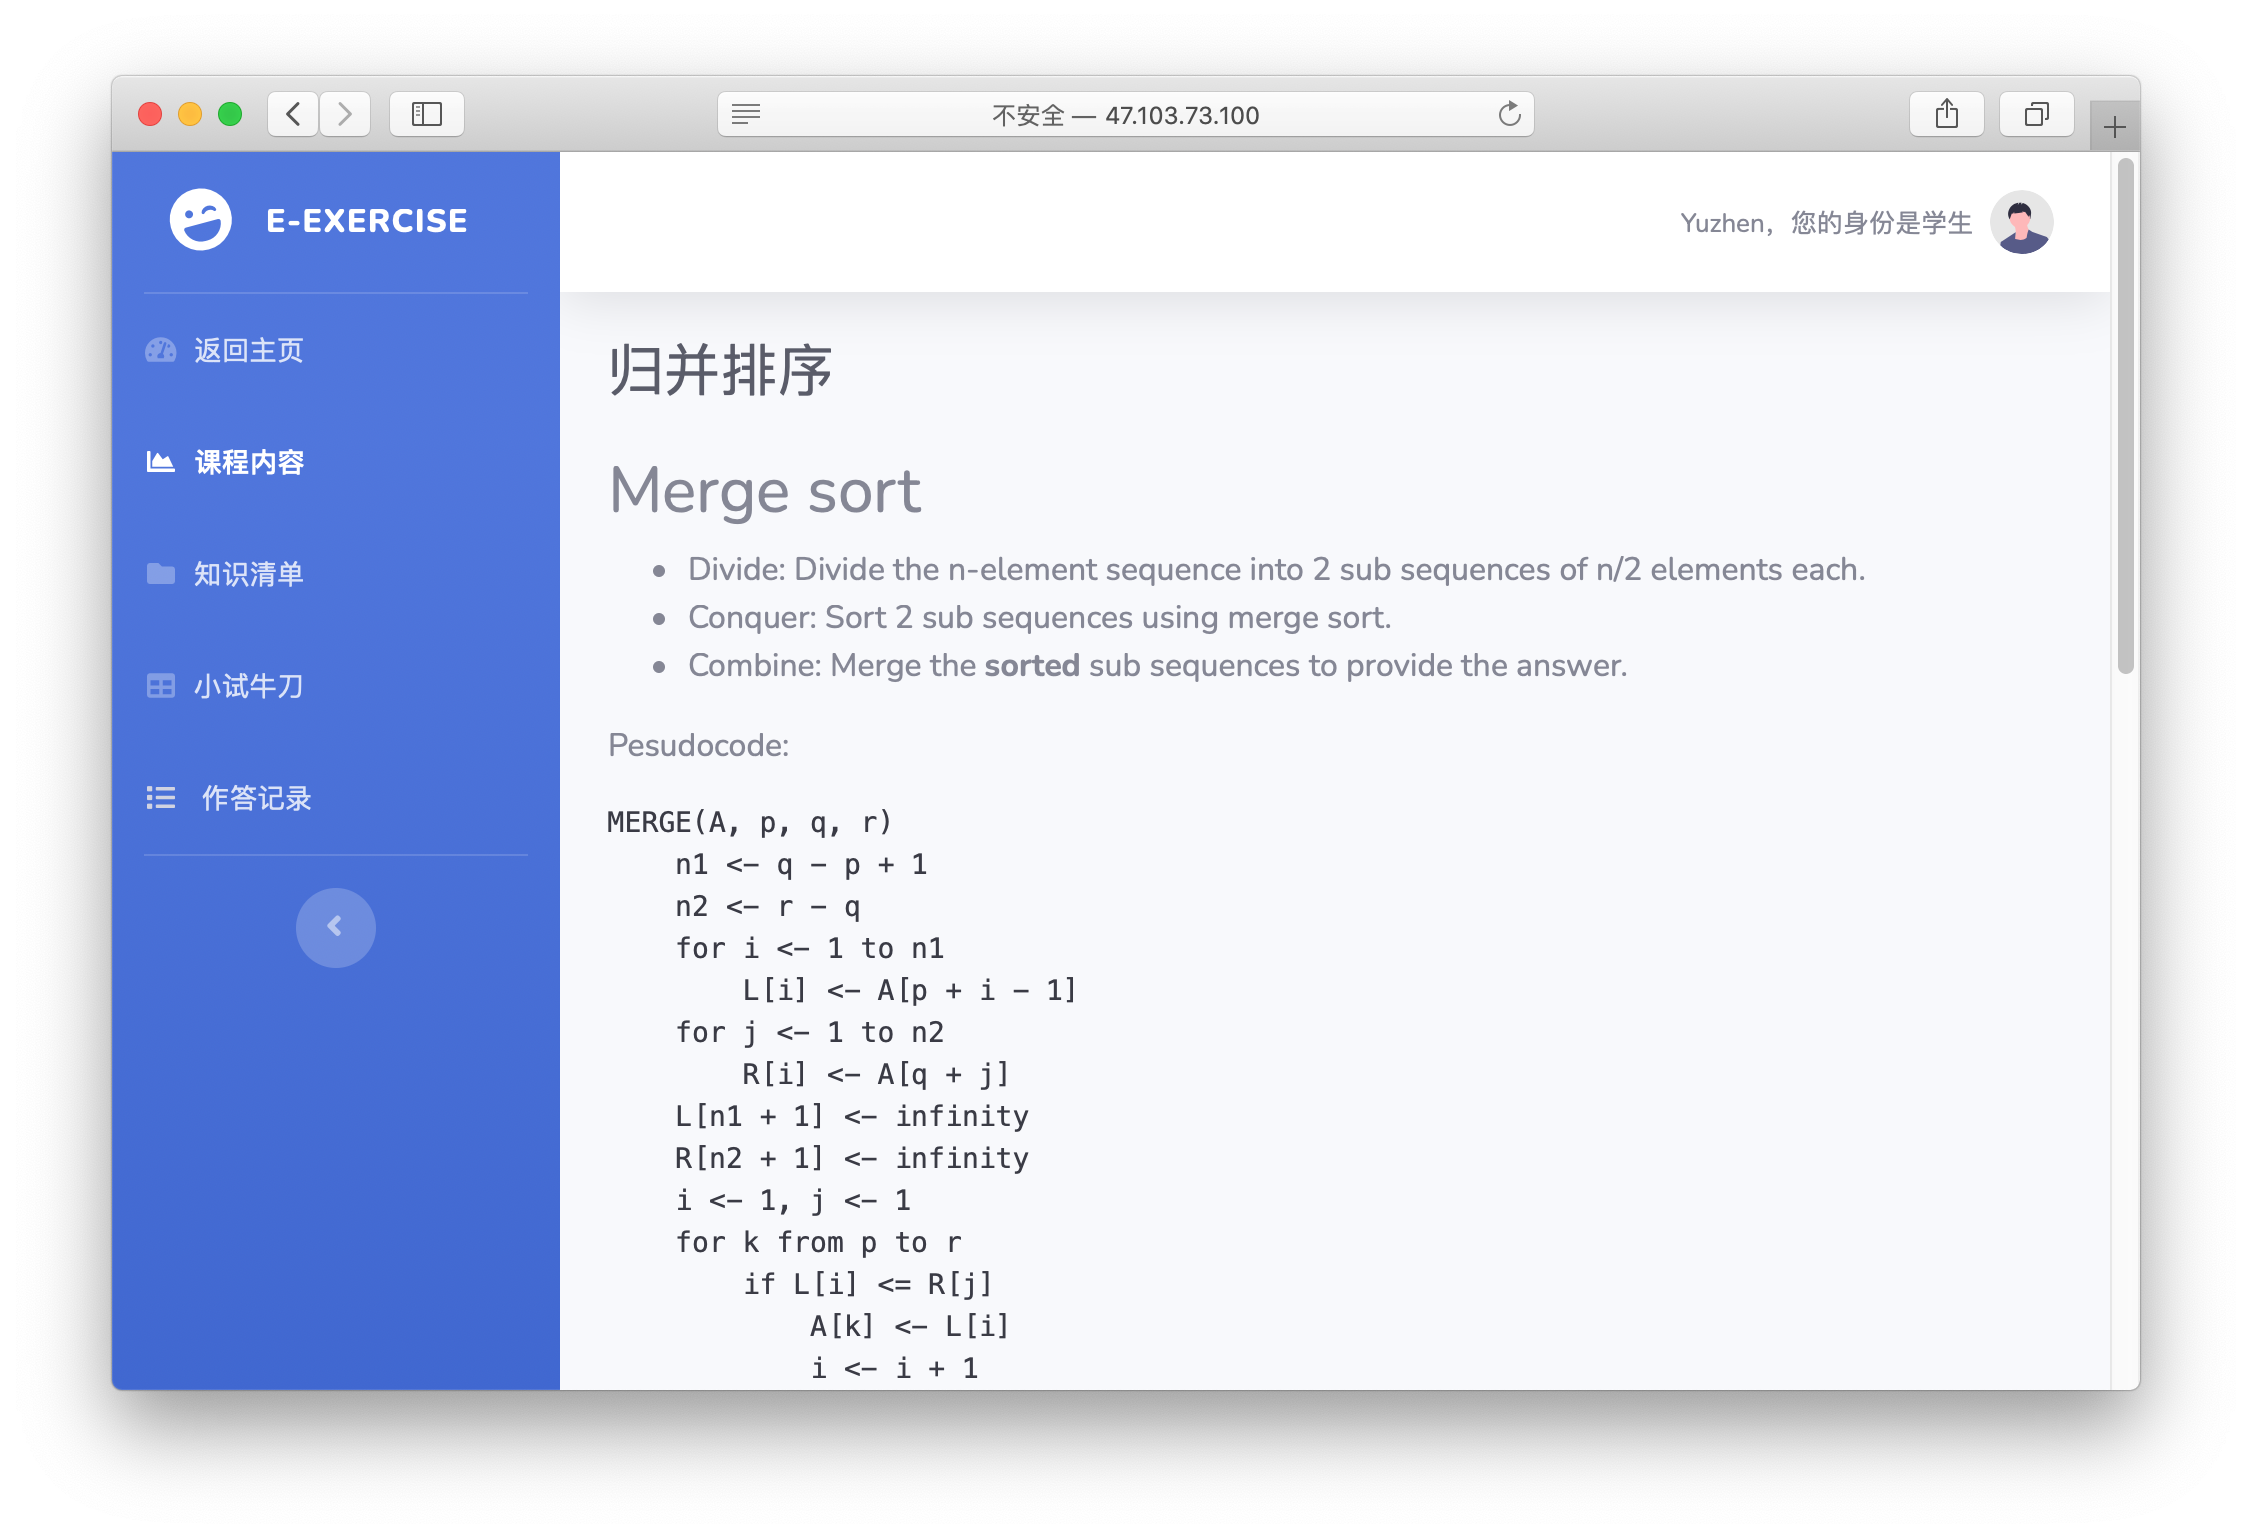
\includegraphics[width=0.8\textwidth]{knowledge_code.png}
  \caption{知识页面——代码}
  \label{knowledge_code}
\end{figure}

\begin{figure}[htp]
  \centering
  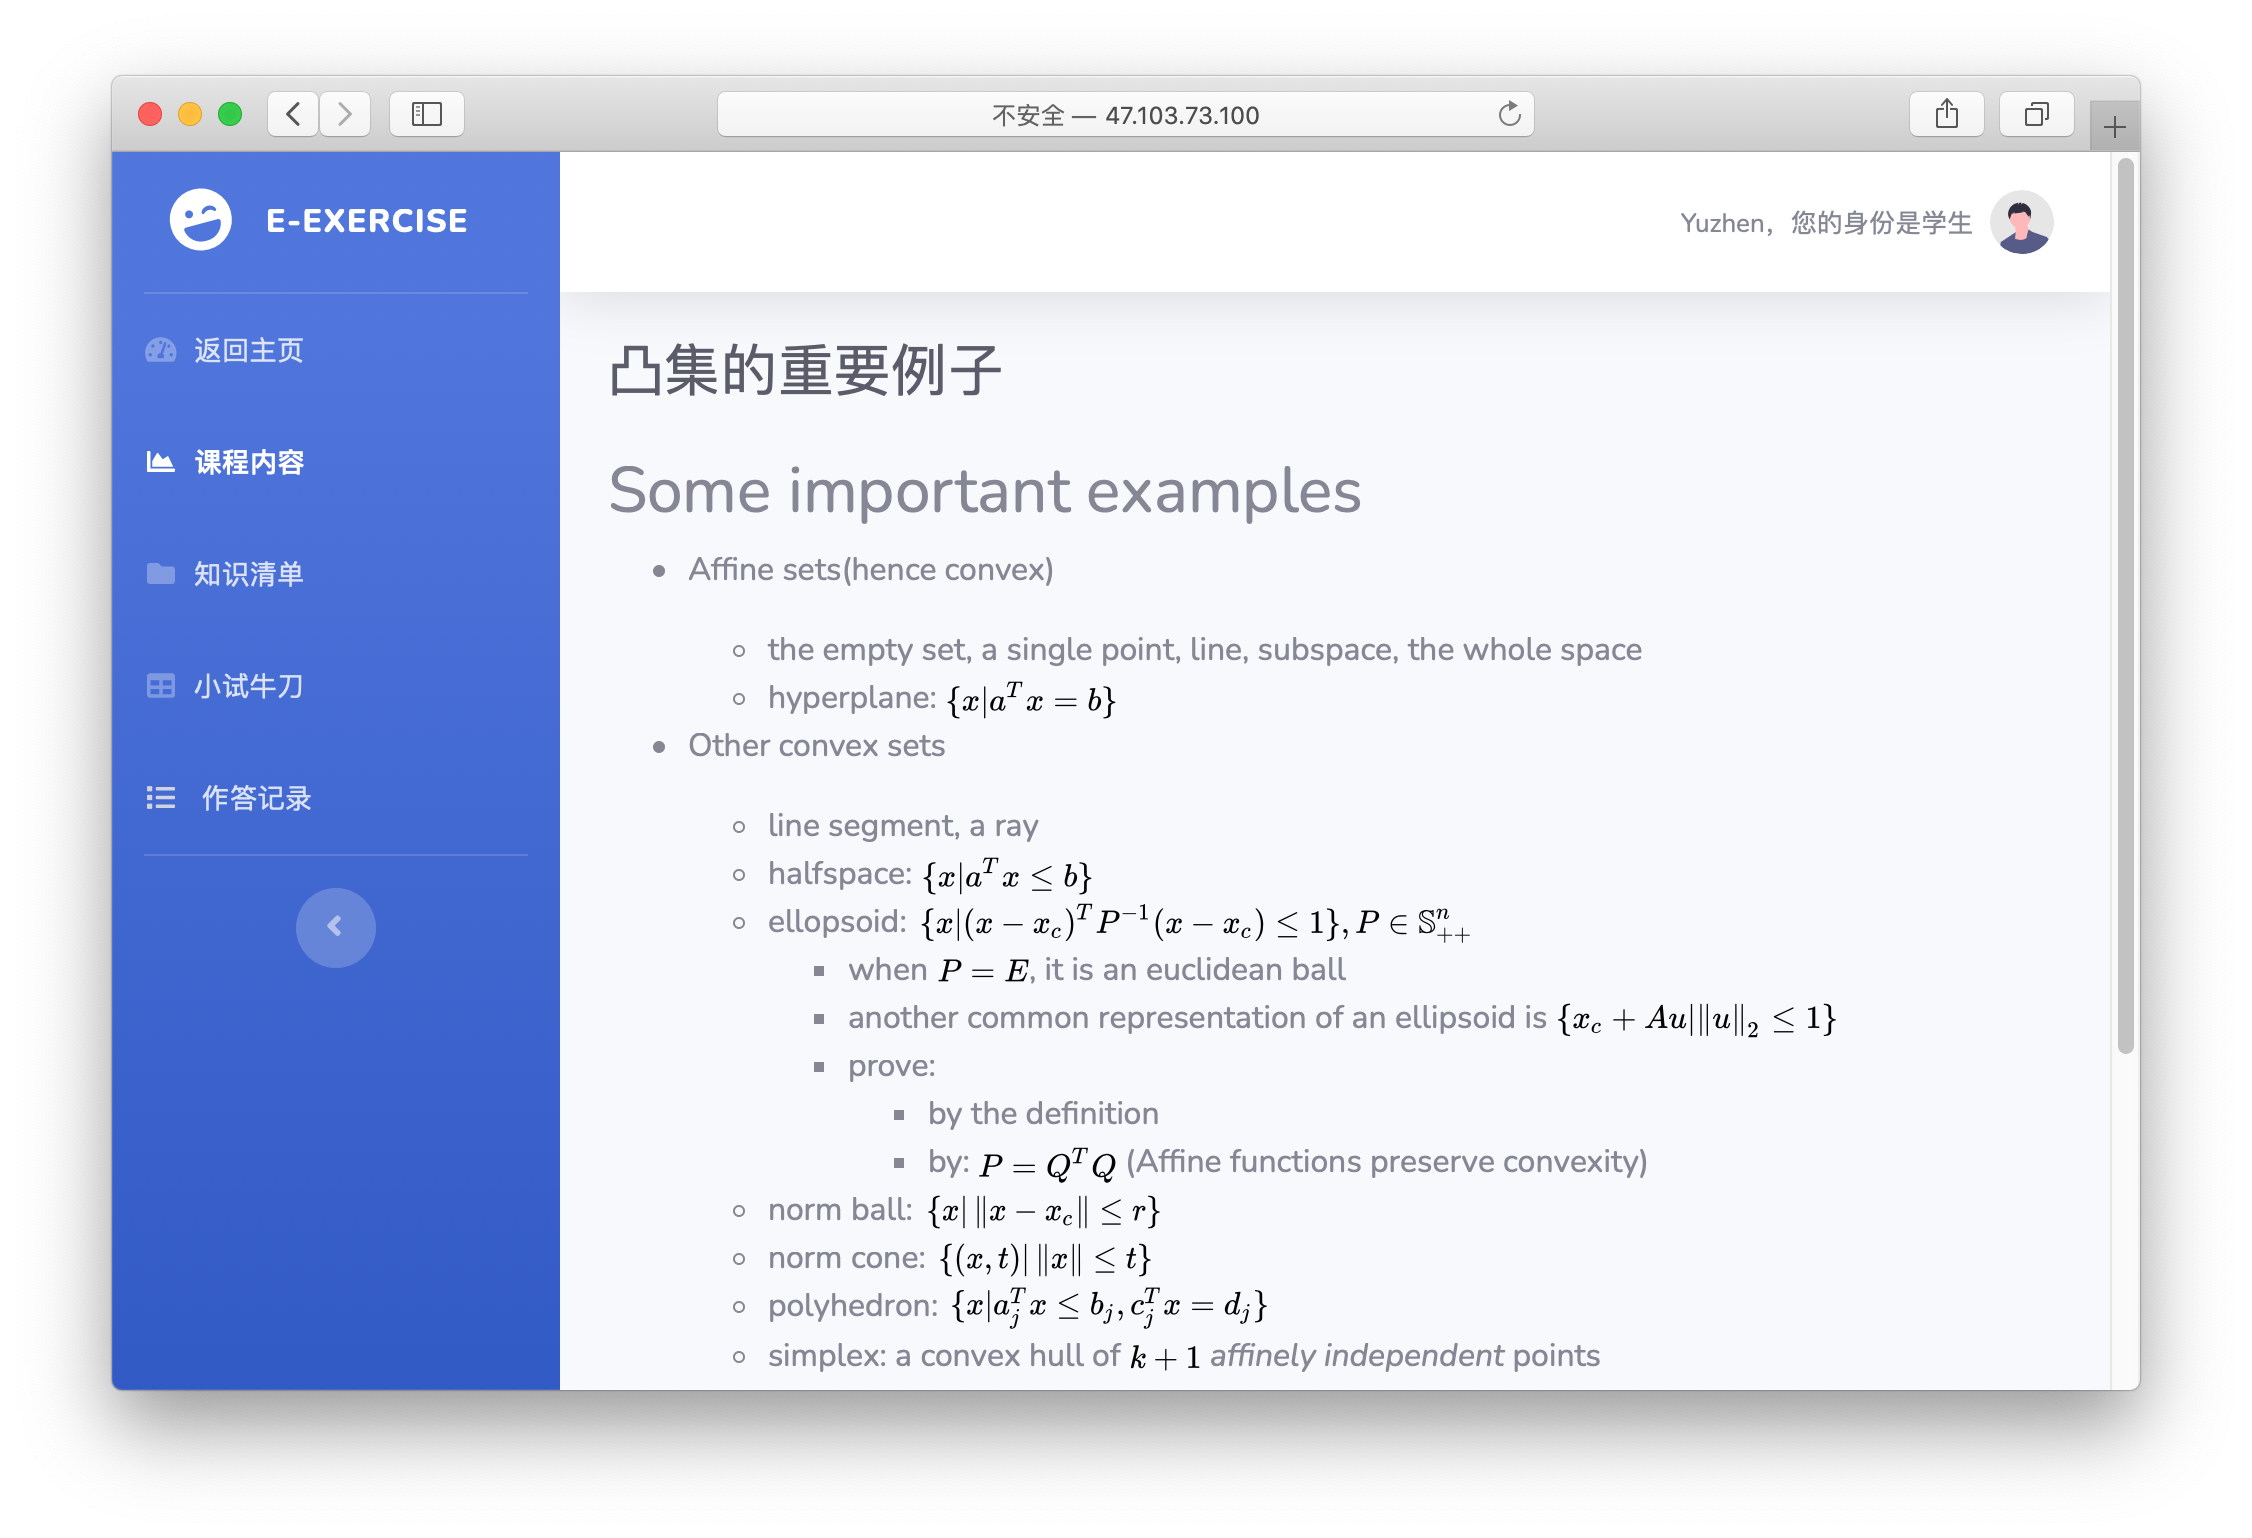
\includegraphics[width=0.8\textwidth]{knowledge_math.png}
  \caption{知识页面——公式}
  \label{knowledge_math}
\end{figure}

\begin{figure}[htp]
  \centering
  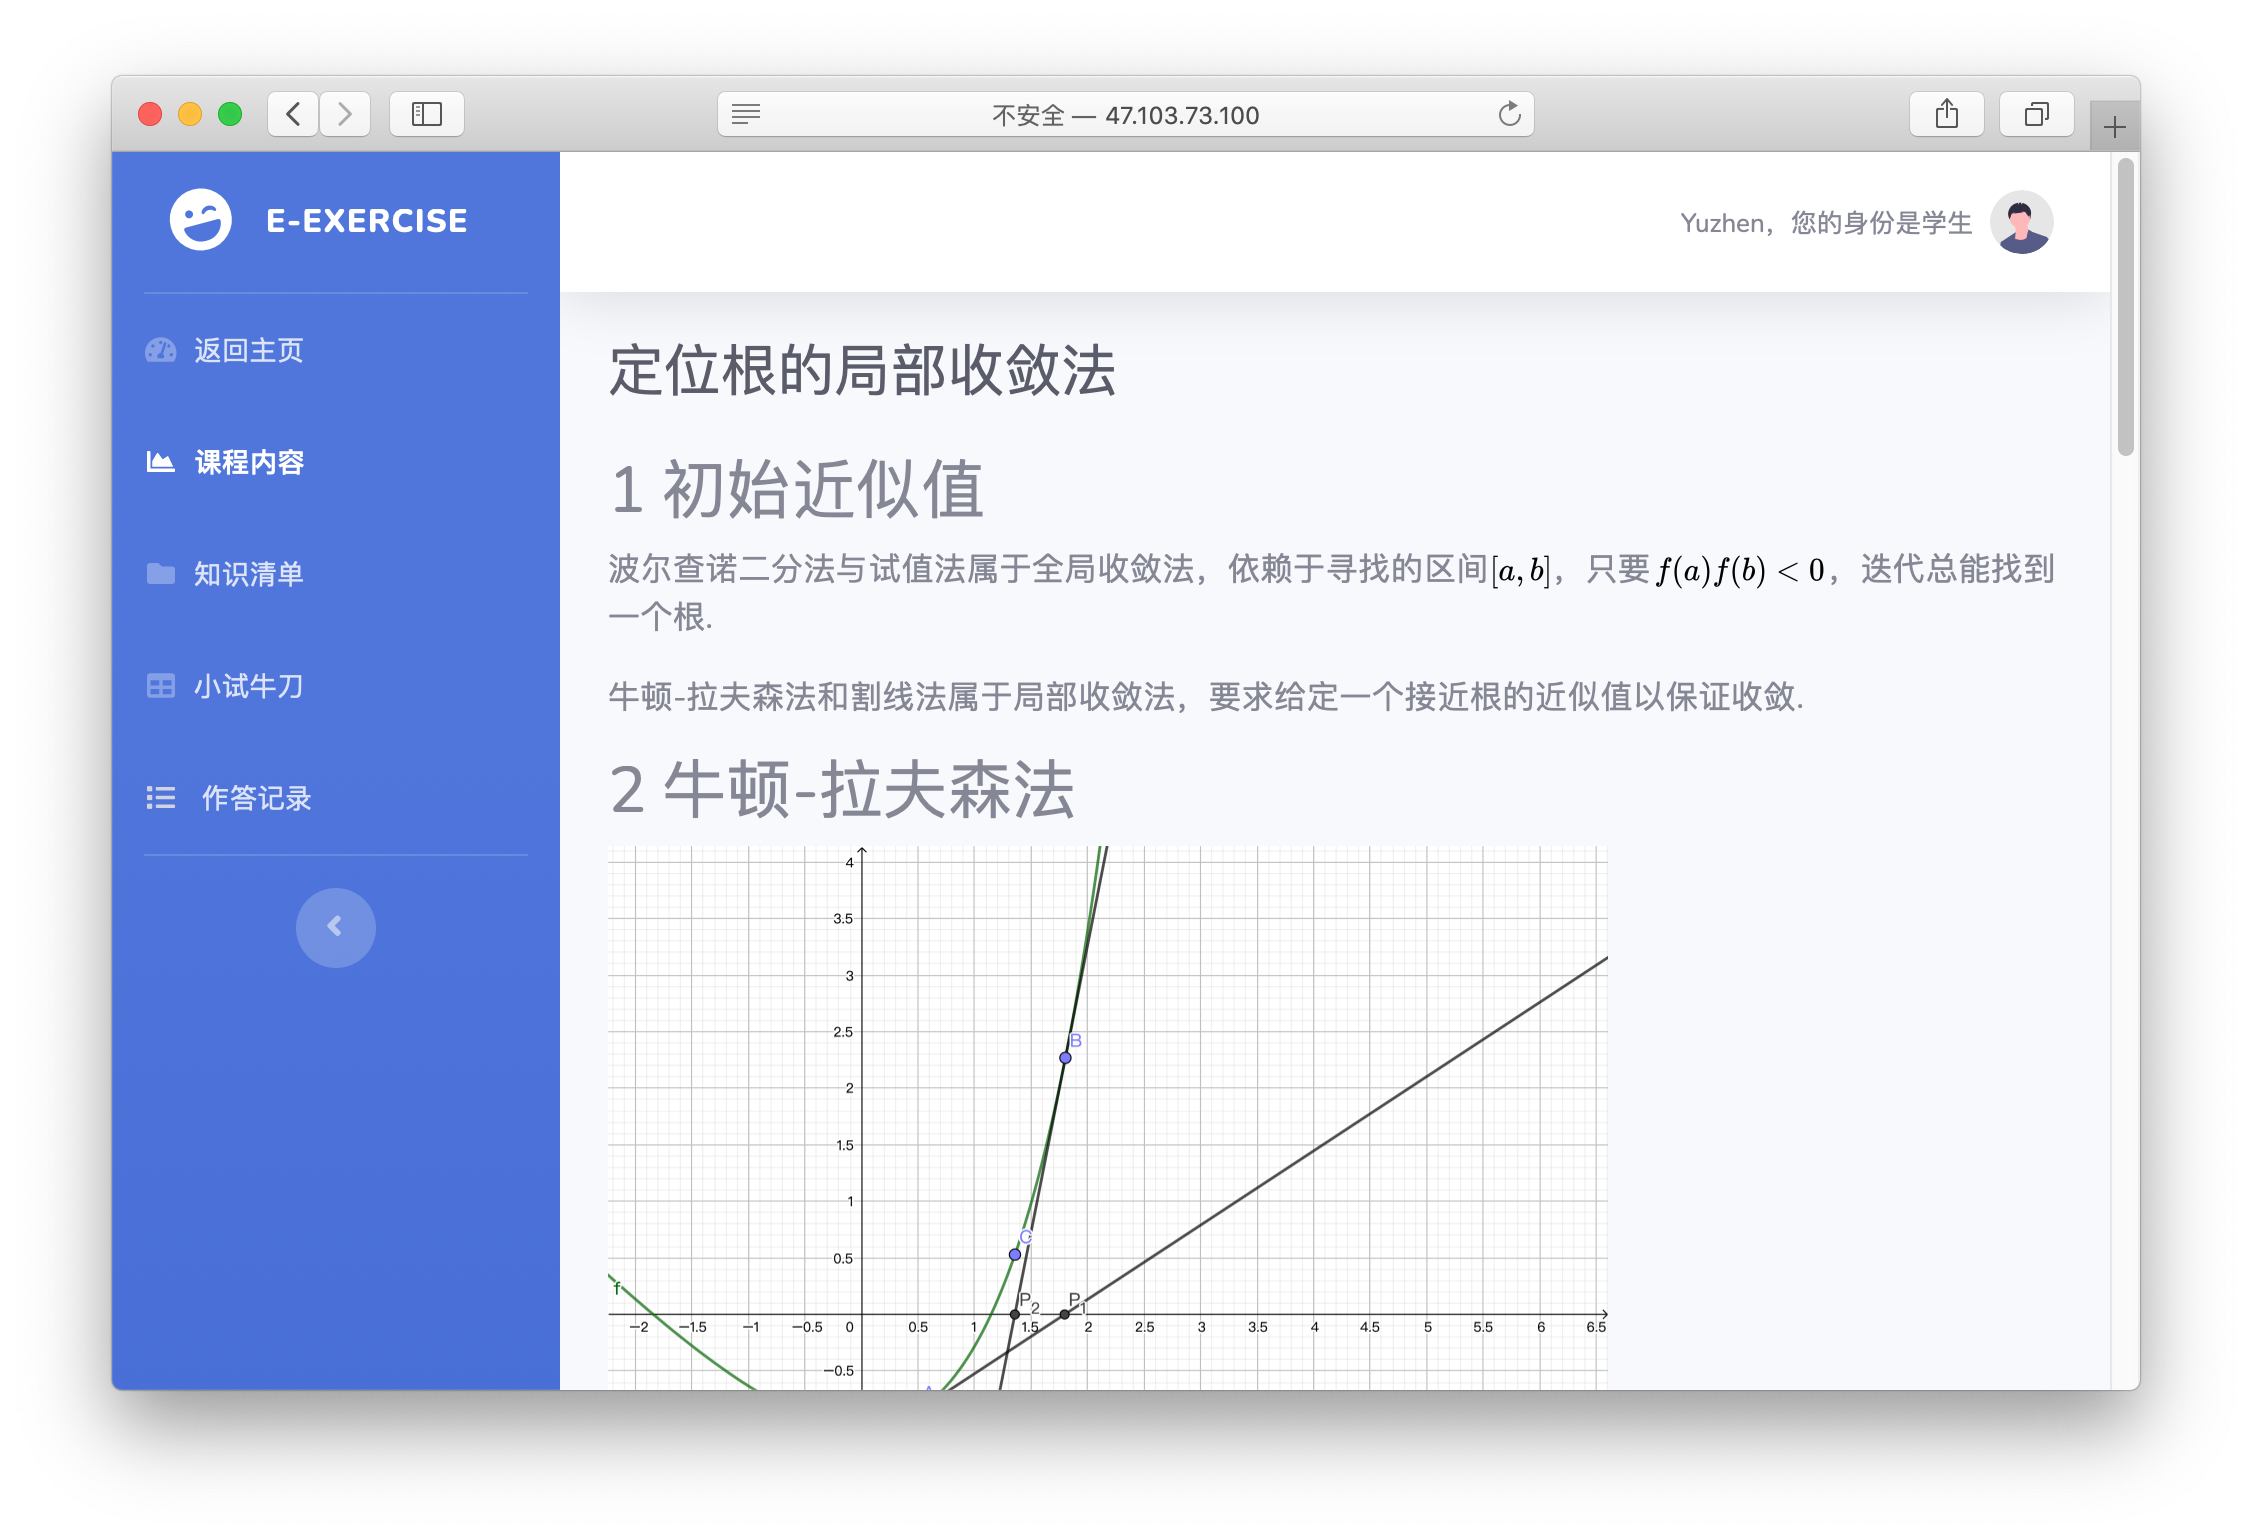
\includegraphics[width=0.8\textwidth]{knowledge_image.png}
  \caption{知识页面——图片}
  \label{knowledge_image}
\end{figure}

知识内容采用Markdown标记语言作为模板,前端可以对符合Markdown语法的内容进行渲染,包括:\textbf{标题、代码、图片等};数学公式使用Zhihu提供的接口,将Tex公式转化为图片(也可使用MathJax,但是很丑陋,故抛弃)。下面展示几种具有代表性的知识页面,如图\ref{knowledge_code}、\ref{knowledge_math}和\ref{knowledge_image}所示。

\begin{figure}[htp]
  \centering
  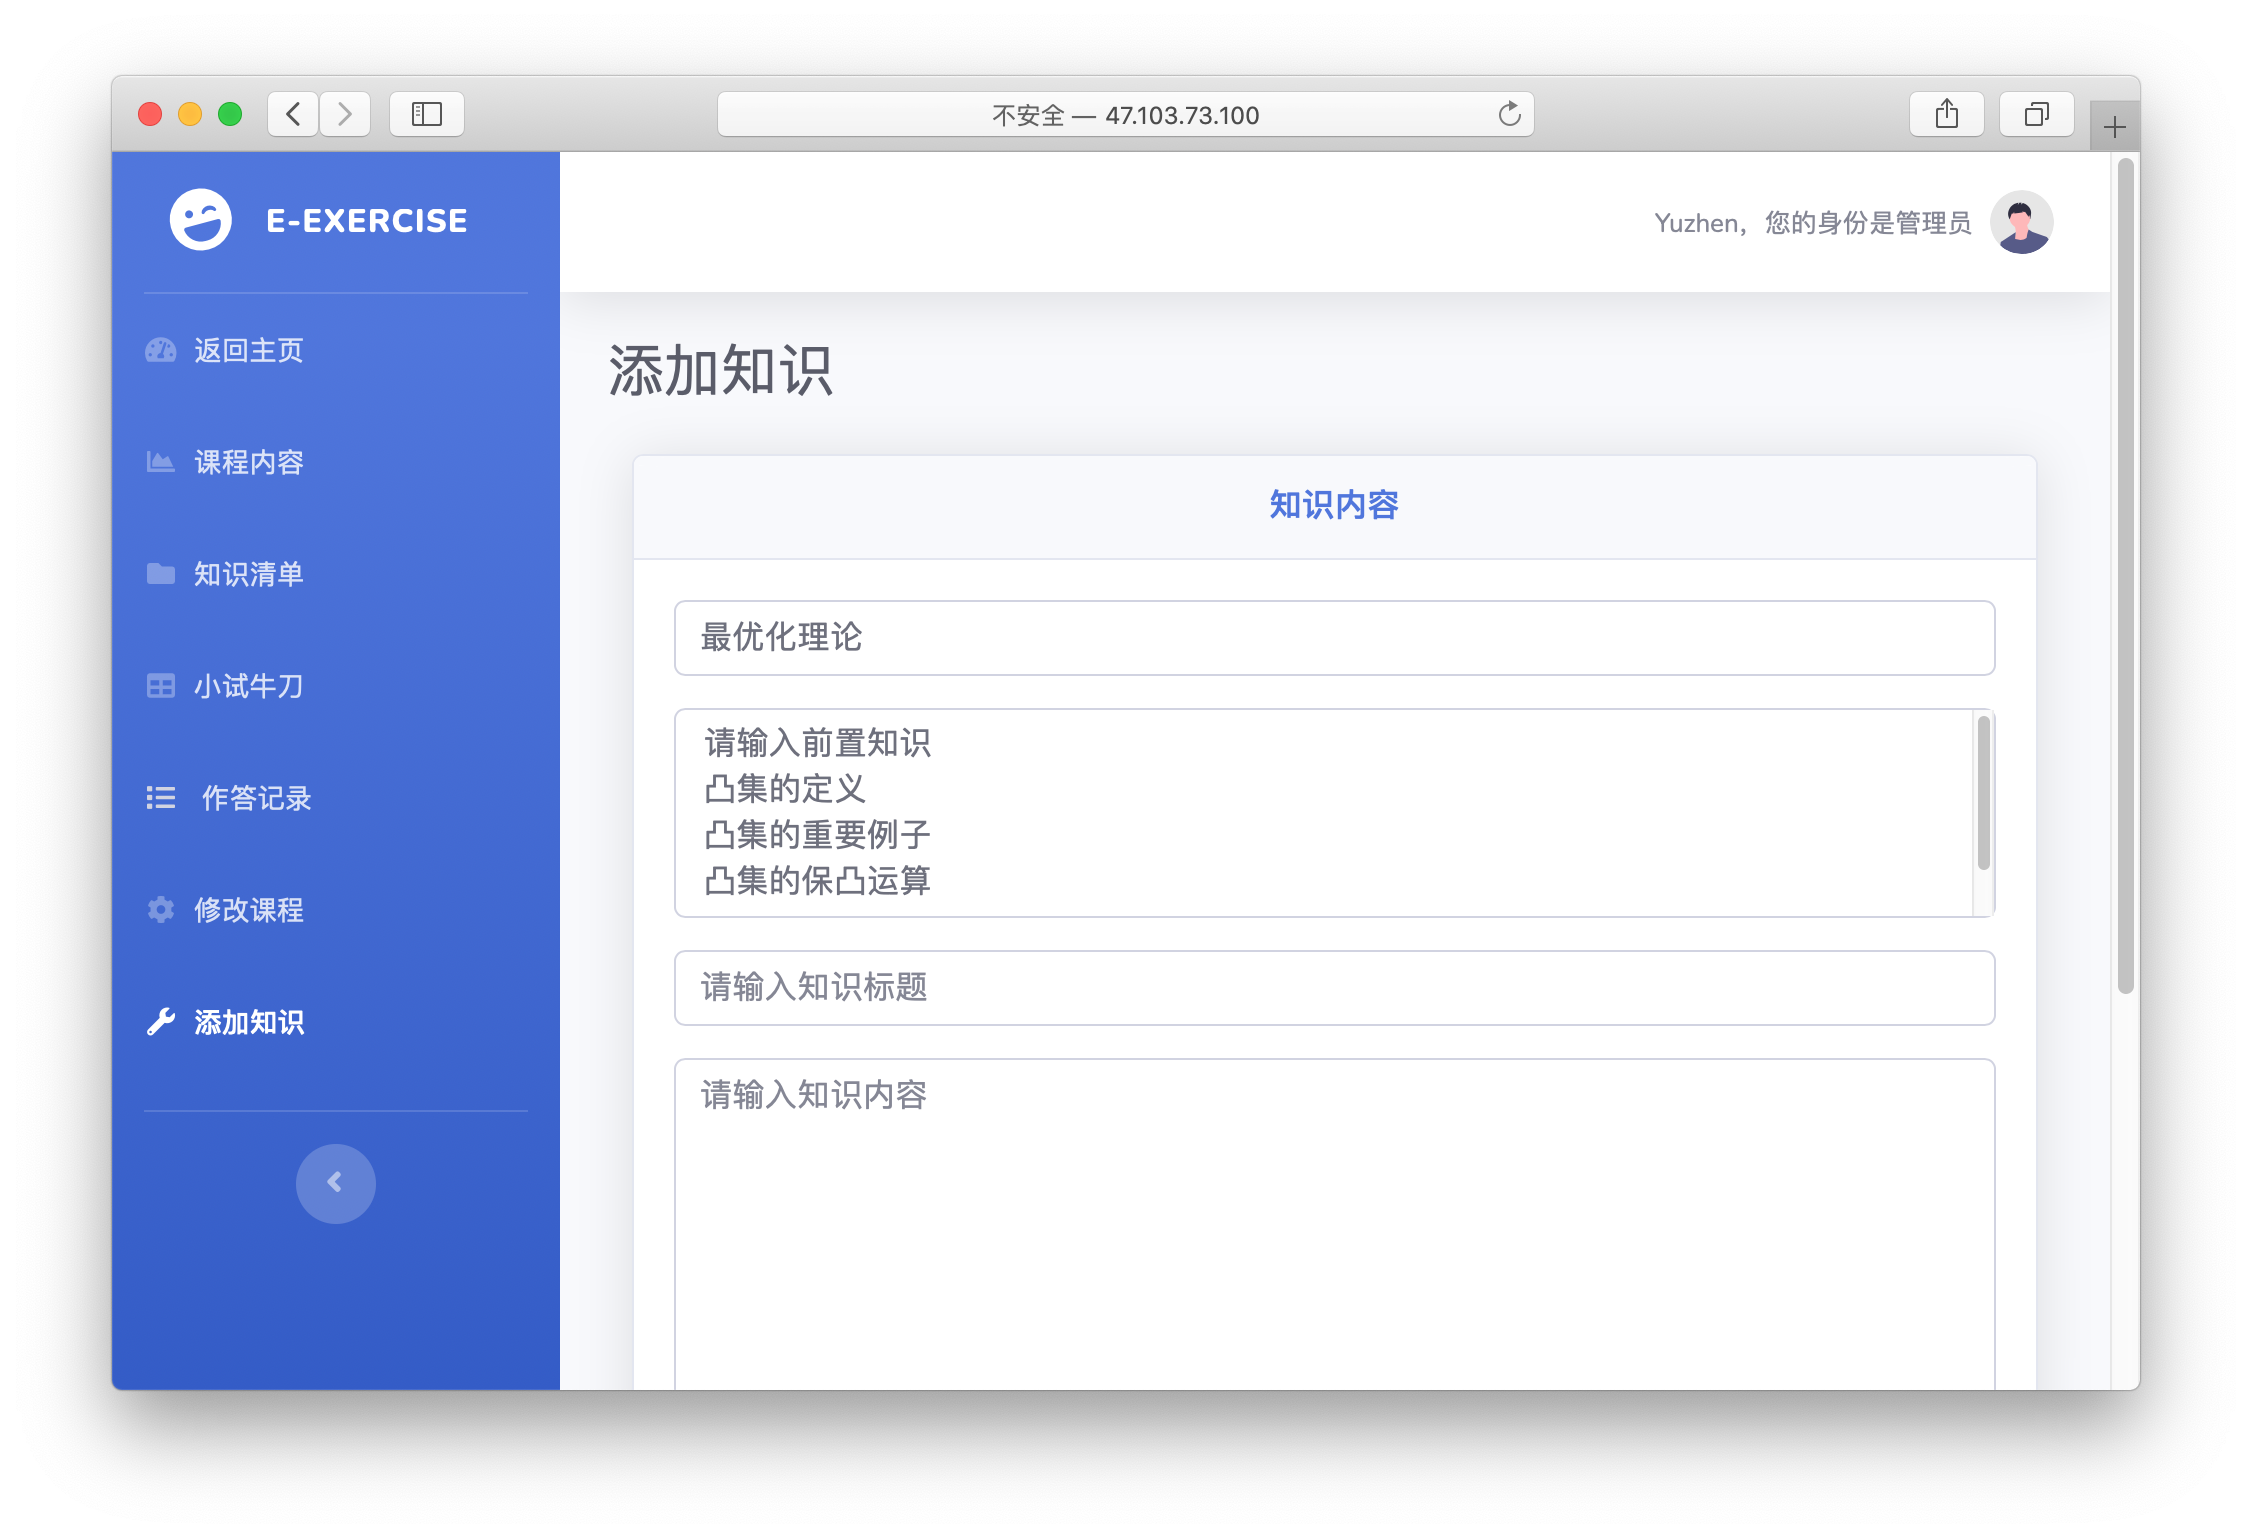
\includegraphics[width=0.8\textwidth]{add_knowledge.png}
  \caption{添加知识}
  \label{add_knowledge}
\end{figure}

\begin{figure}[htp]
  \centering
  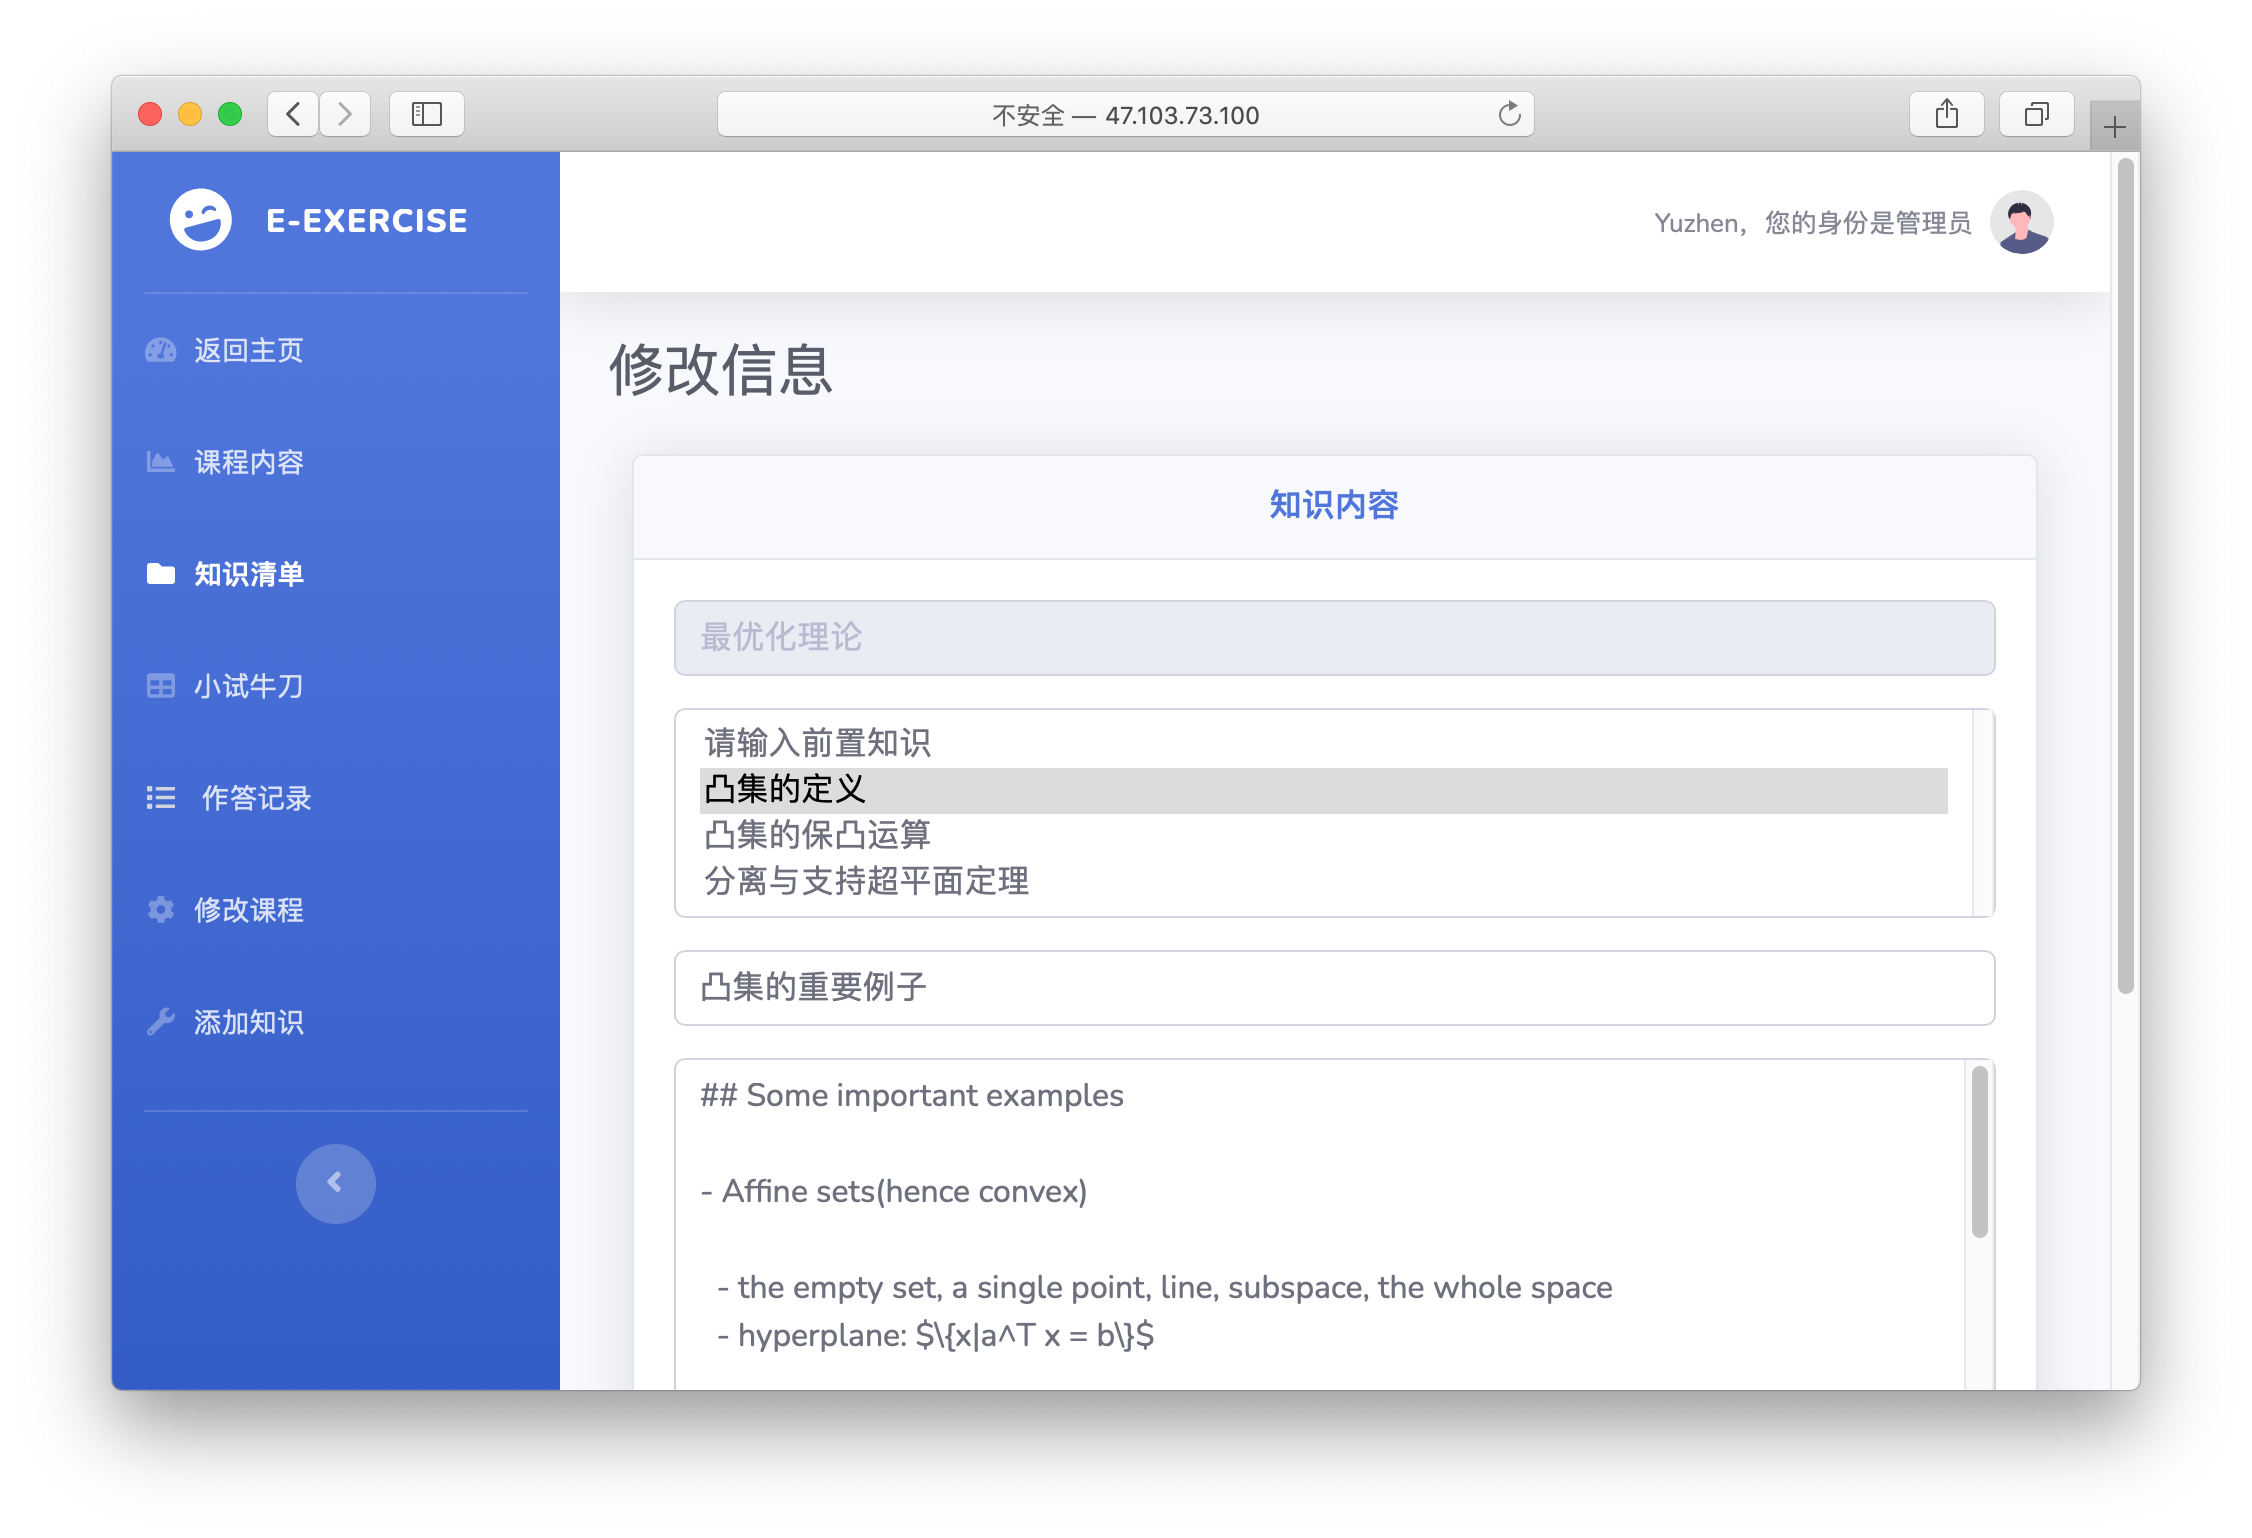
\includegraphics[width=0.8\textwidth]{modify_knowledge.png}
  \caption{修改知识}
  \label{modify_knowledge}
\end{figure}

对于管理员与教师来说,可以添加课程、添加知识、修改课程、修改知识等。简便起见,这里仅展示添加和修改知识,添加和修改课程相对来说更加简单。添加和修改知识时,可以为该知识增加前置依赖知识,两功能的界面如图\ref{add_knowledge}和\ref{modify_knowledge}所示。

\begin{figure}[htp]
  \centering
  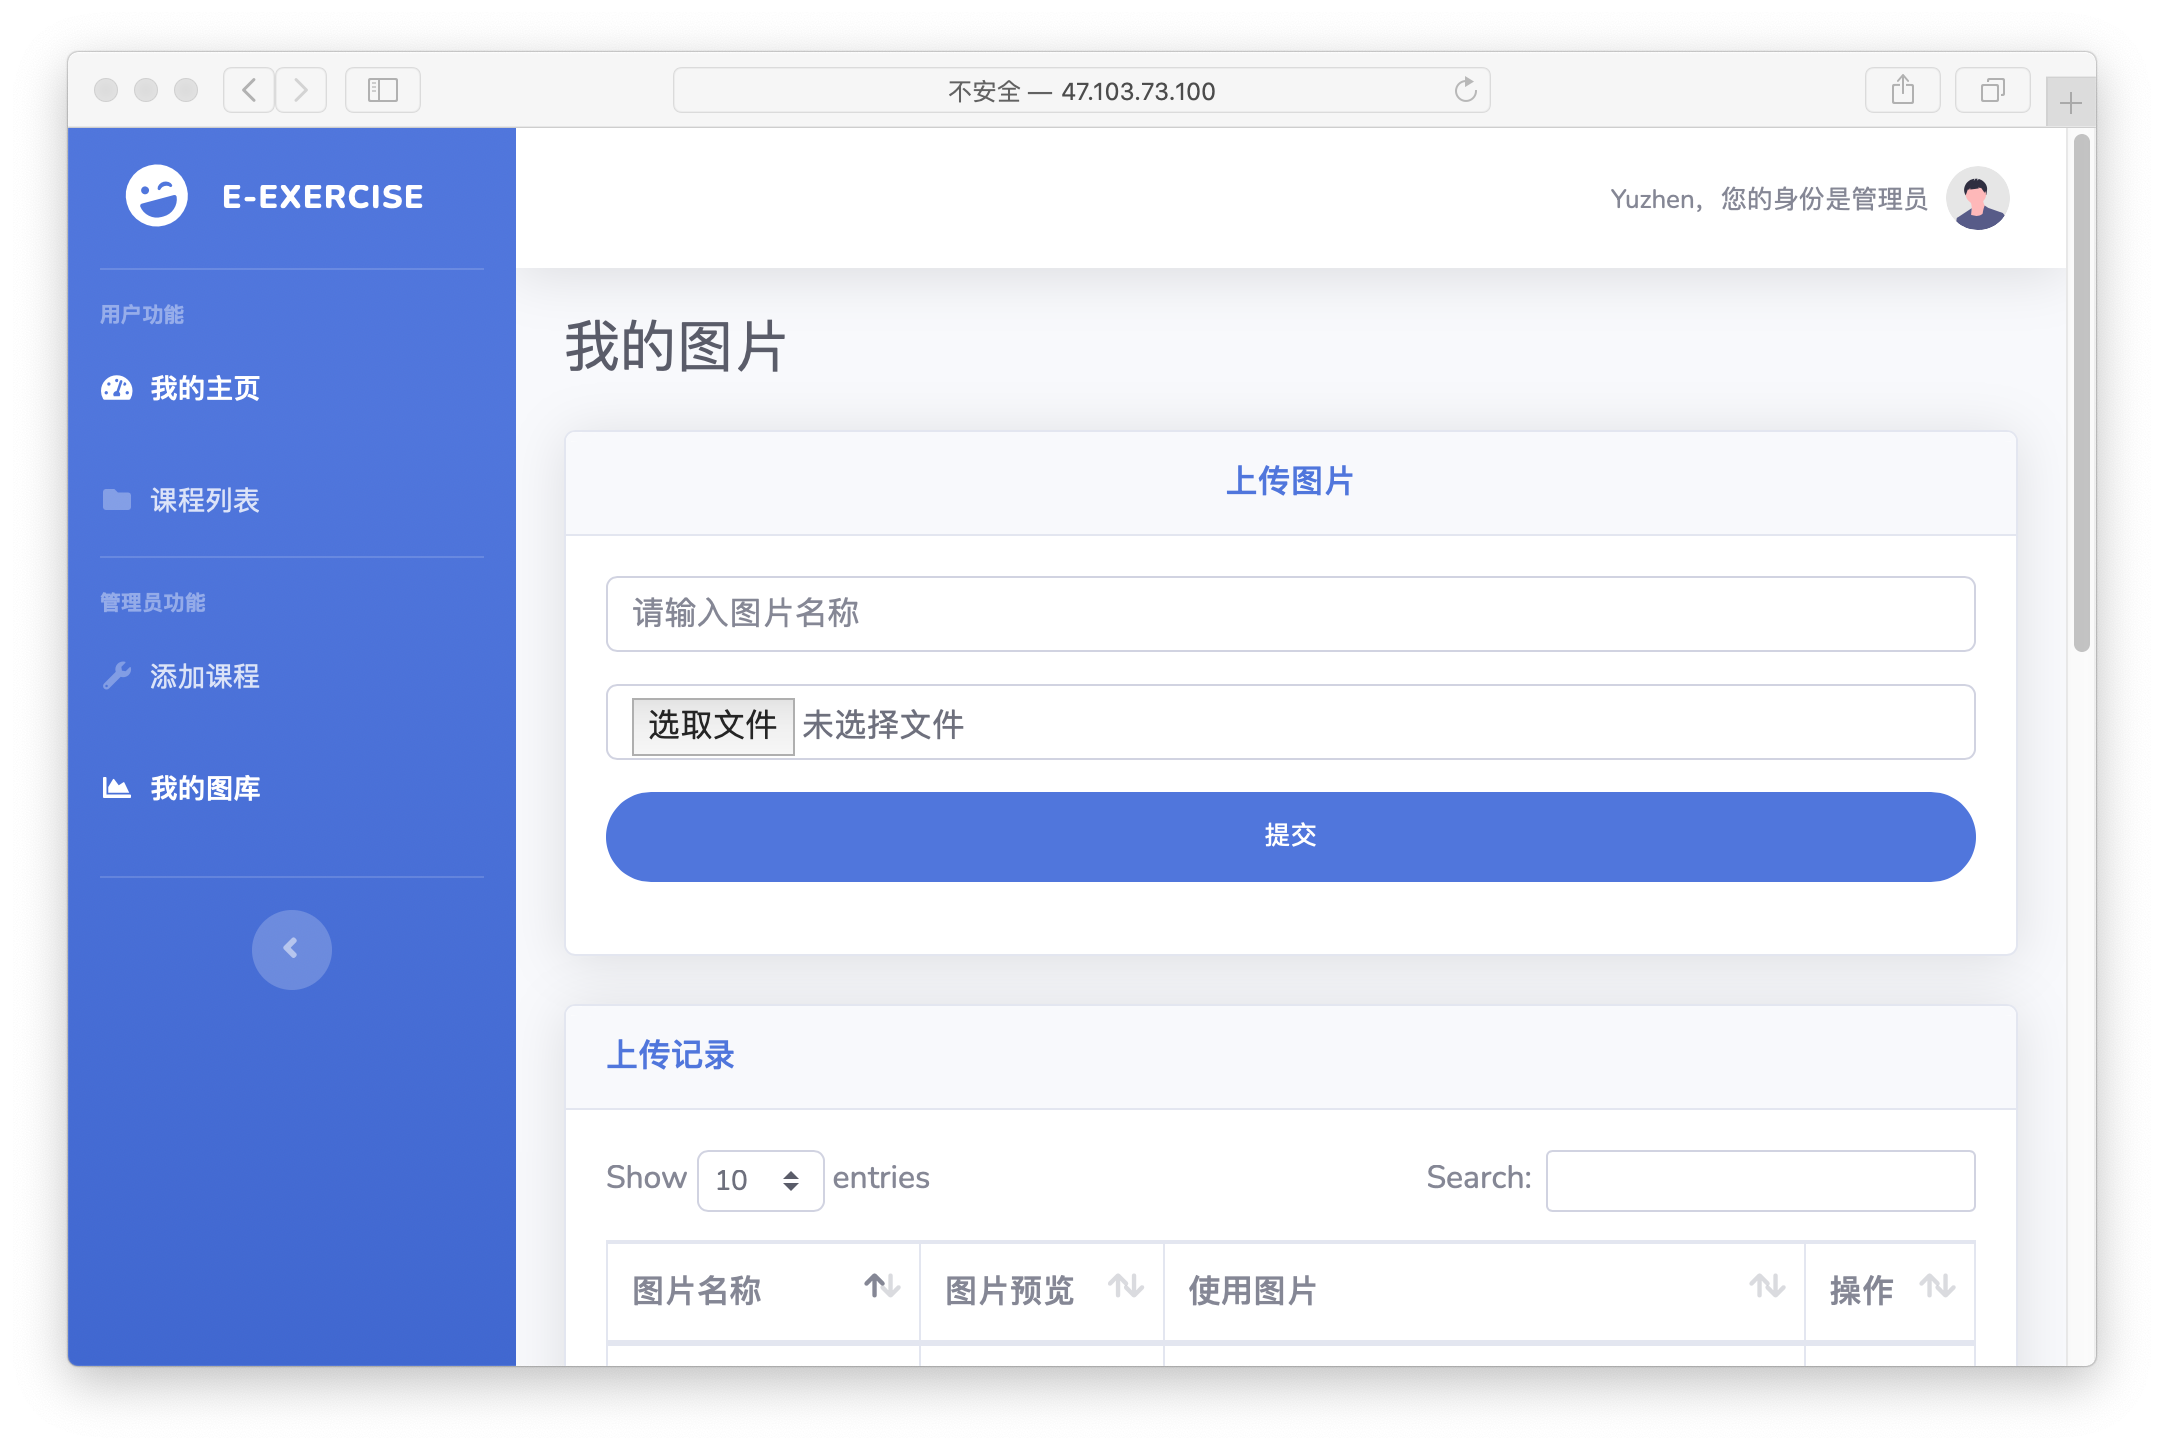
\includegraphics[width=0.8\textwidth]{add_image.png}
  \caption{上传图片}
  \label{add_image}
\end{figure}

\begin{figure}[htp]
  \centering
  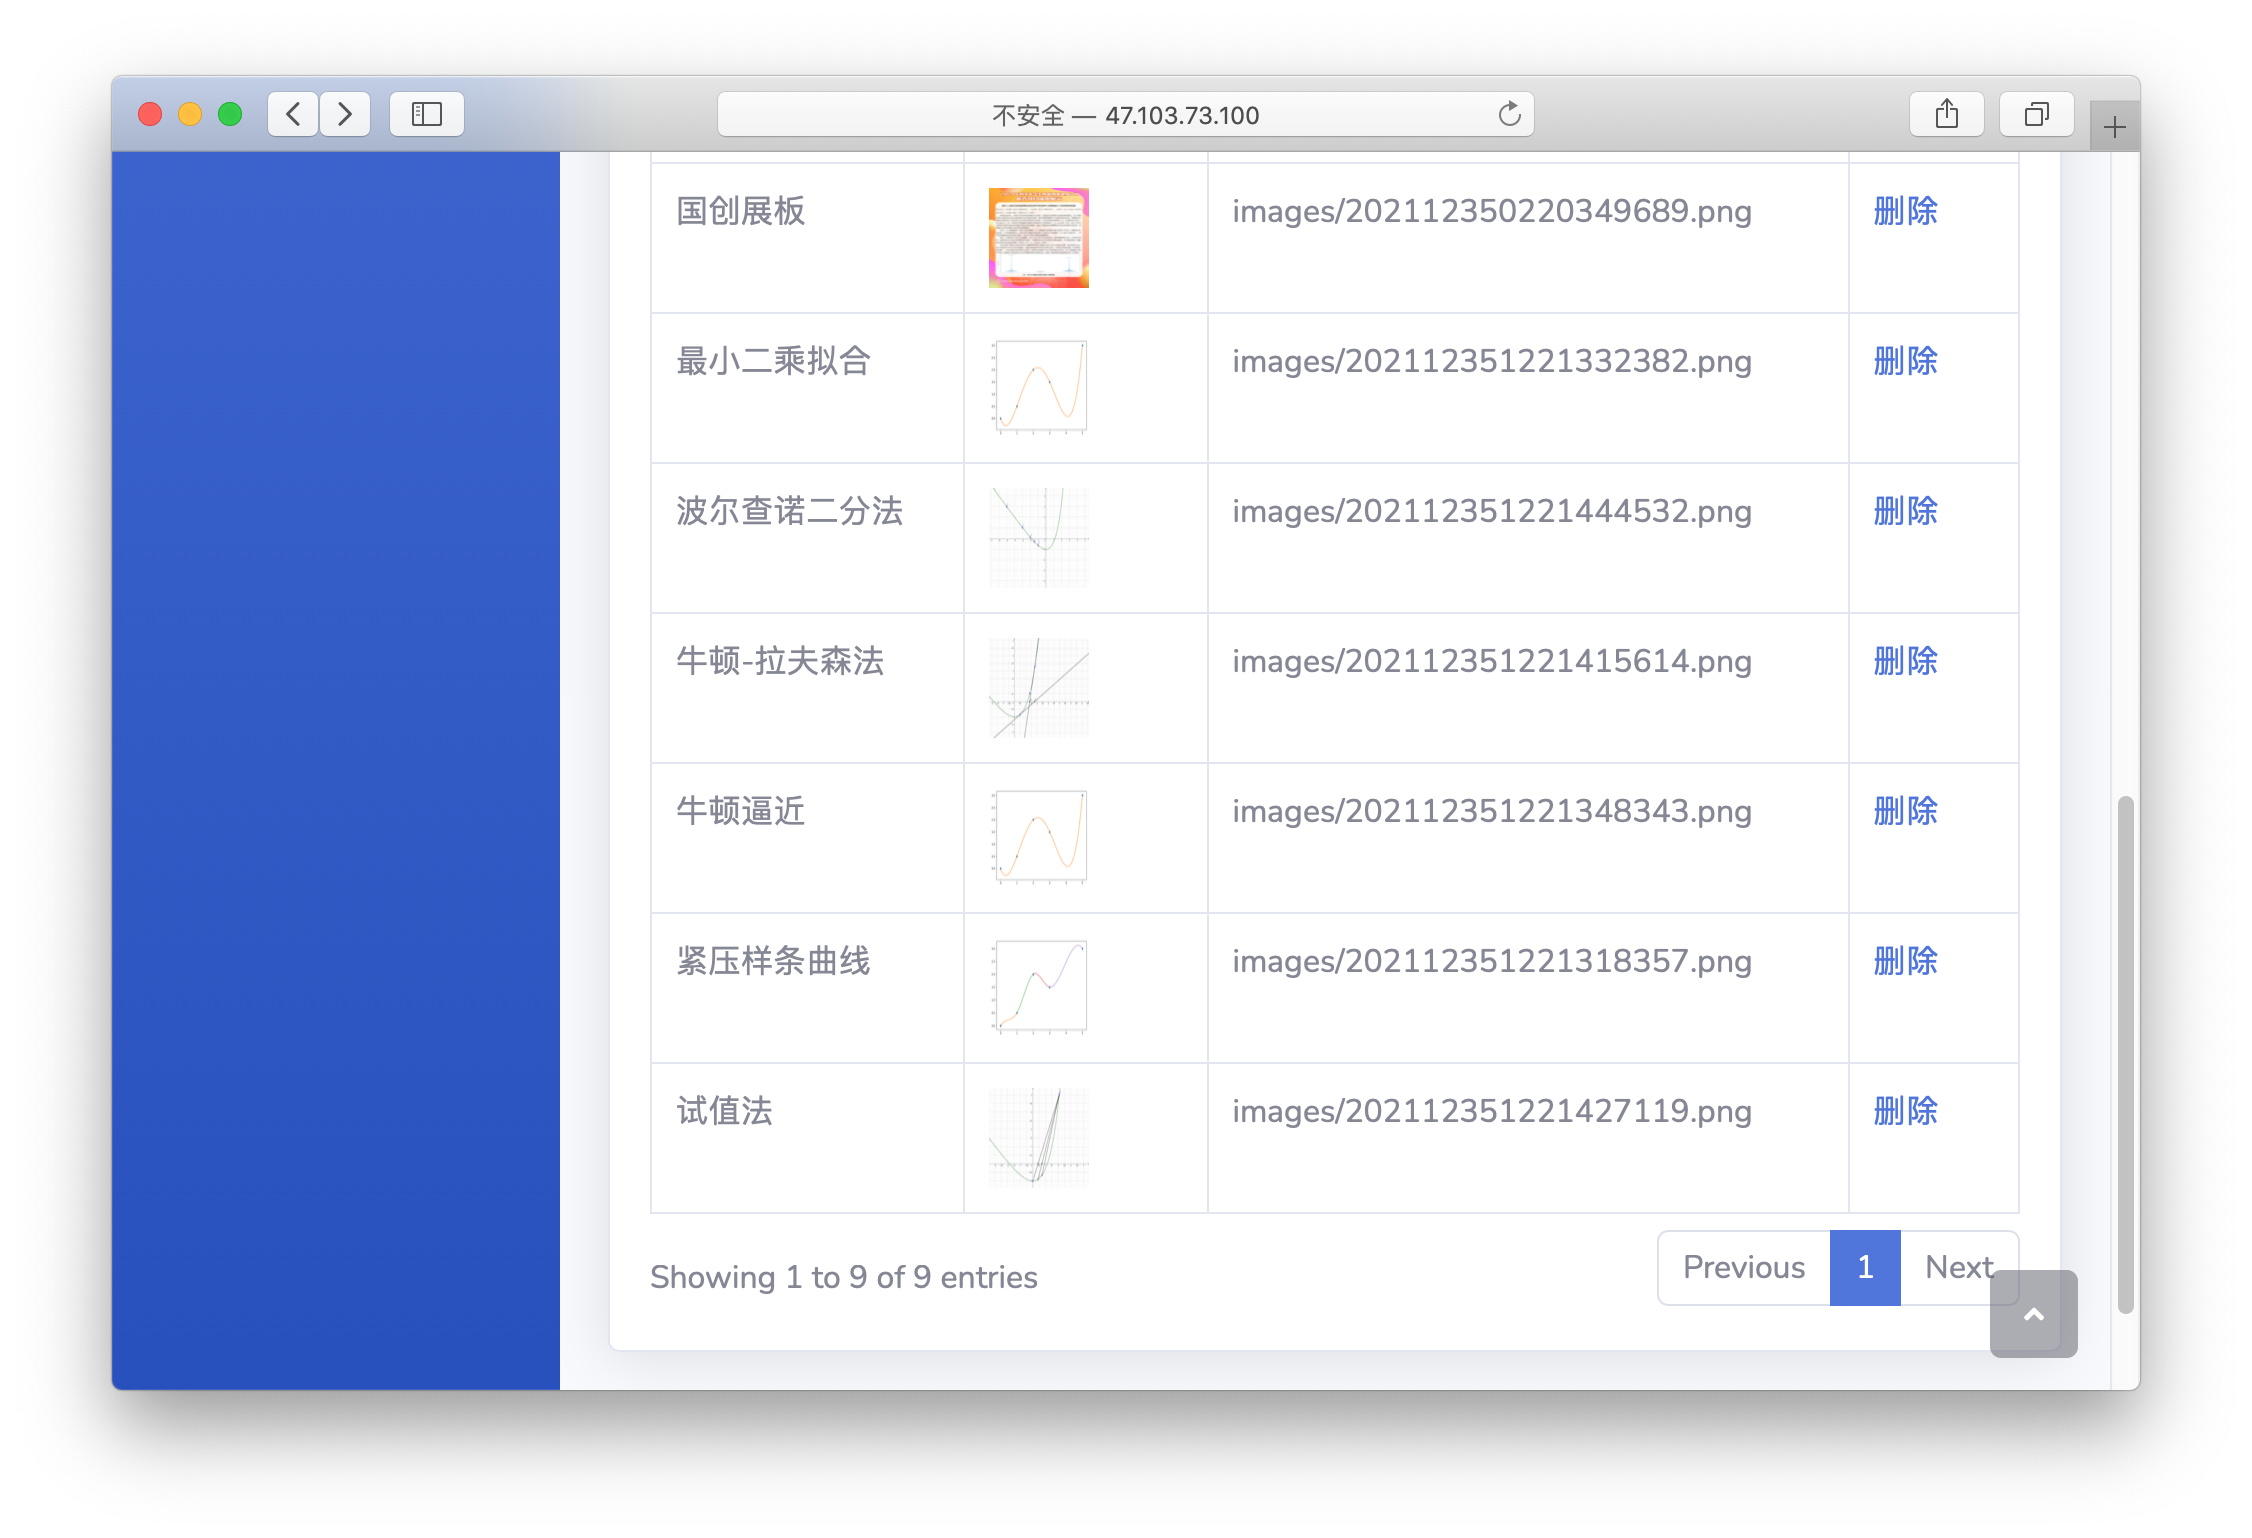
\includegraphics[width=0.8\textwidth]{use_image.png}
  \caption{使用图片}
  \label{use_image}
\end{figure}

为了服务管理员和教师书写知识的需要,本网站添加了“我的图库”功能,可以上传图片,如图\ref{add_image}所示。图片上传后,如图\ref{use_image}所示;通过Markdown或HTML的标记方式可以在知识中使用图片。例如,在图\ref{knowledge_image}所示的页面中,即在知识中插入语句
\begin{lstlisting}
  ![牛顿-拉夫森法](images/202112351221415614.png)
\end{lstlisting}
即可在知识中插入图片。

\newpage

\subsection{习题功能}

\begin{figure}[htp]
  \centering
  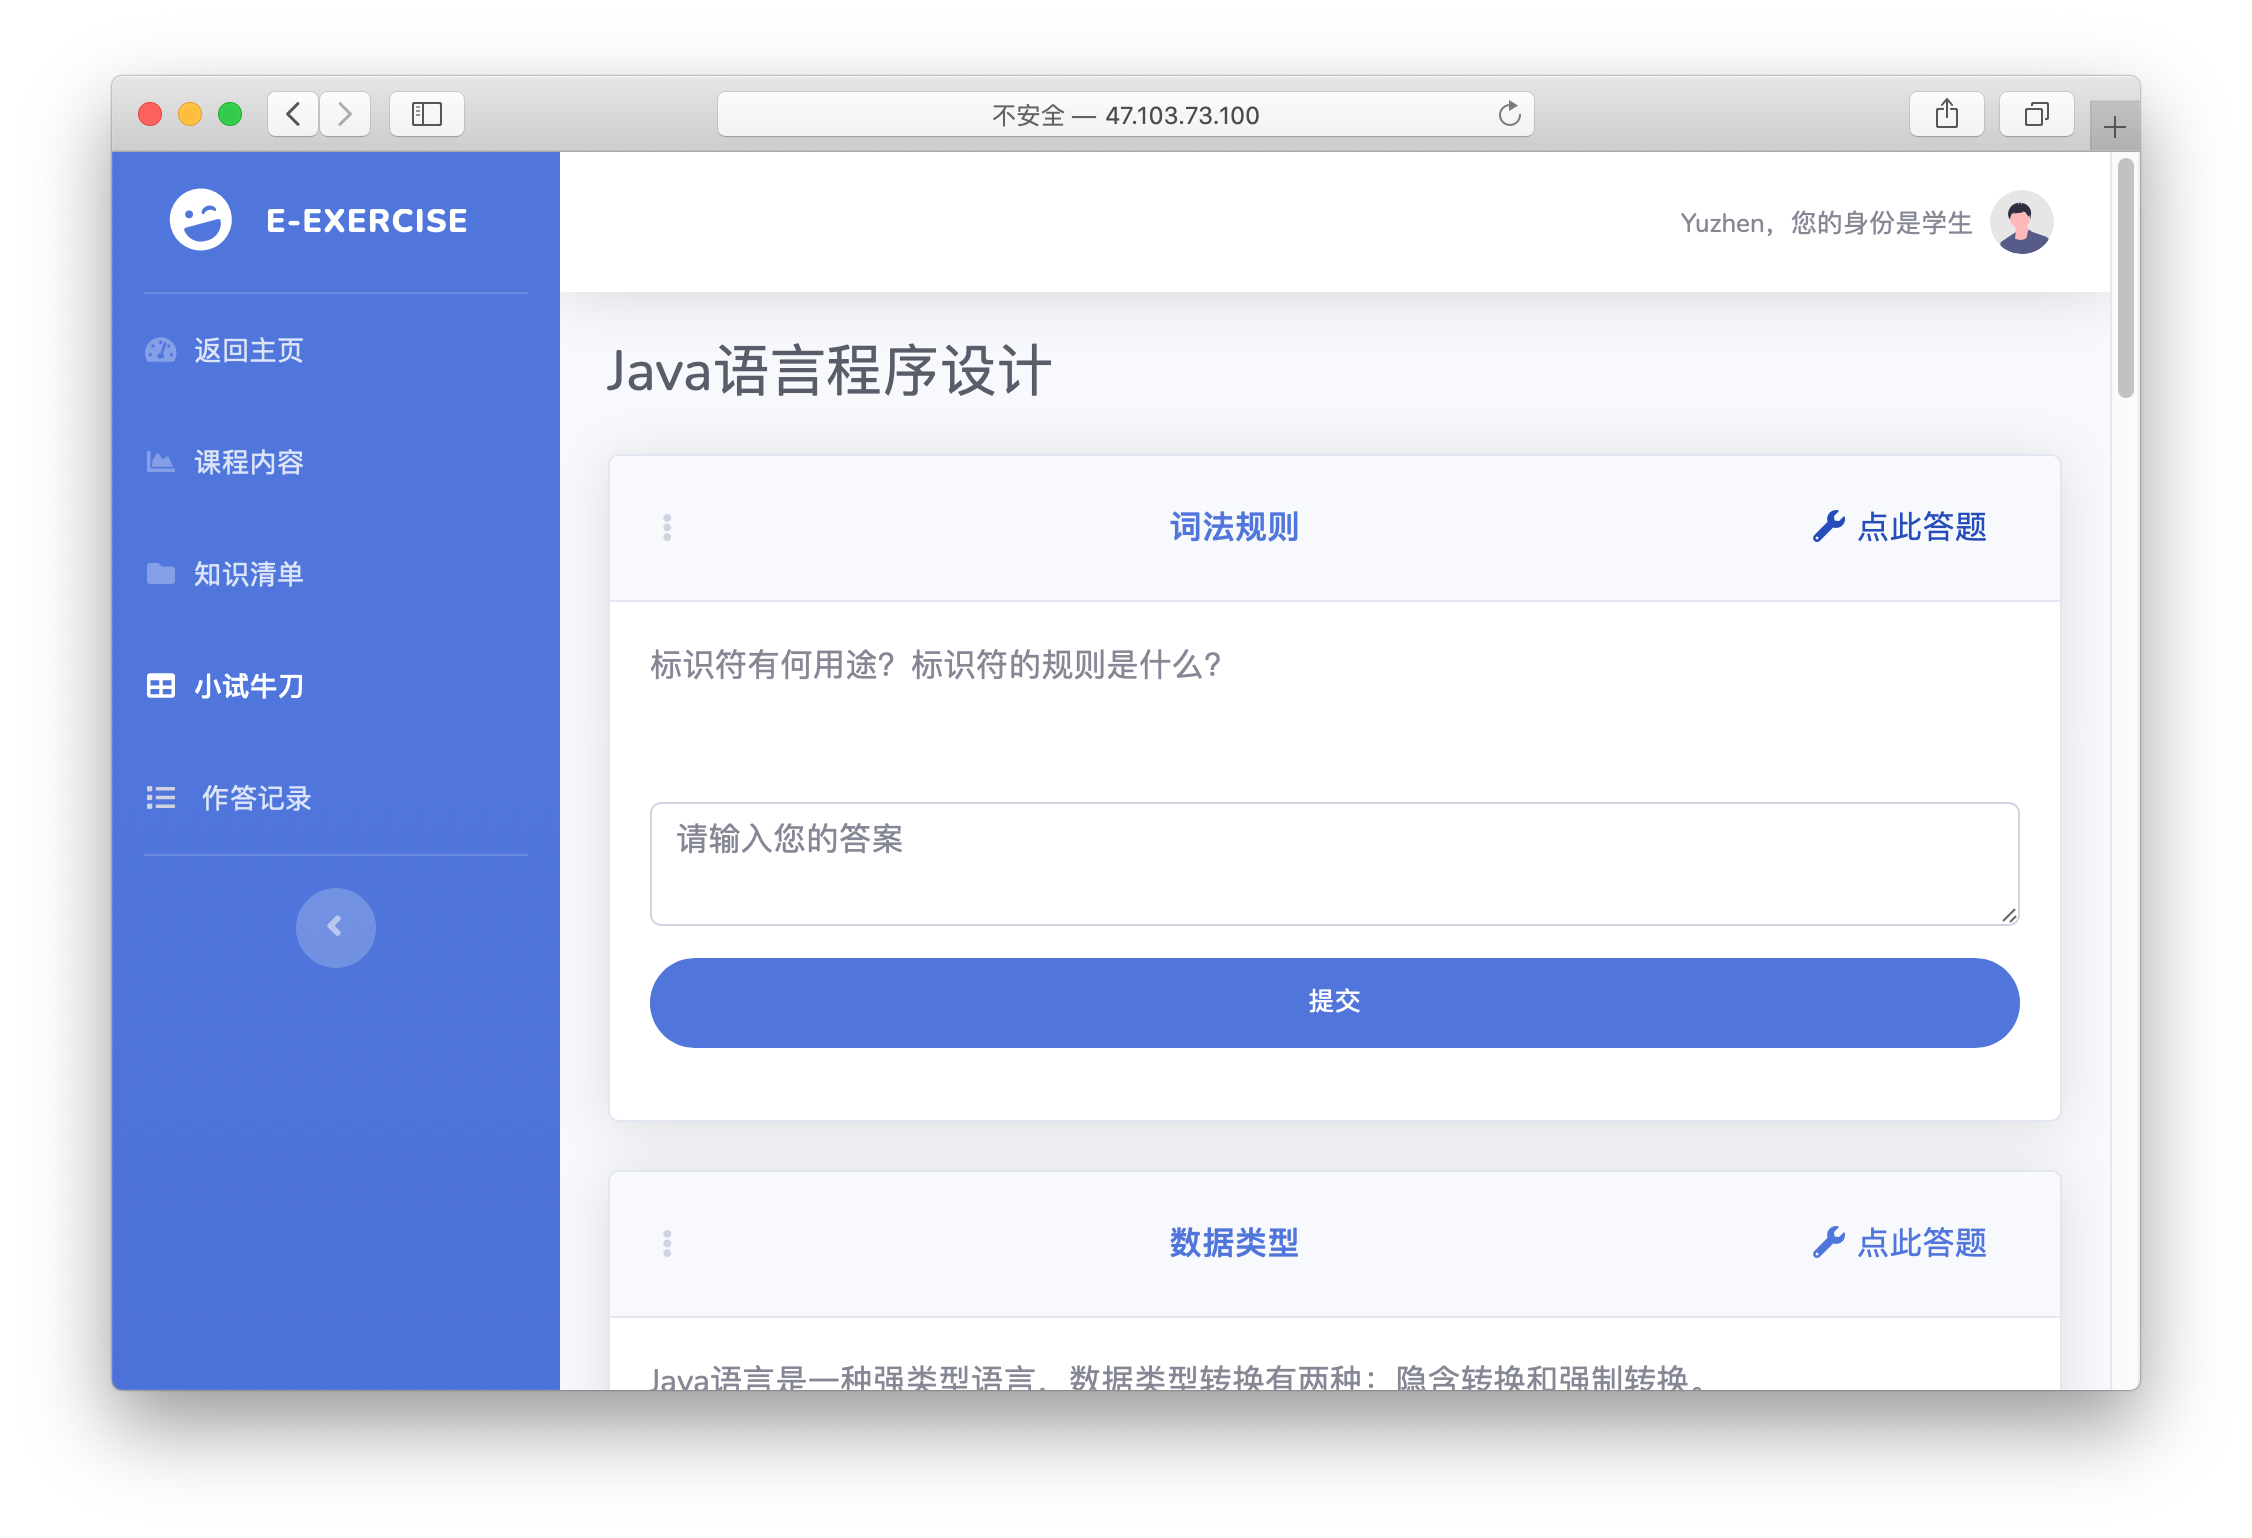
\includegraphics[width=0.8\textwidth]{recommend_exercise.png}
  \caption{习题推荐}
  \label{recommend_exercise}
\end{figure}

对于学生用户来说,进入知识清单后可以查看对应知识的习题,也可以通过“小试牛刀”界面查看系统推荐的习题,如图\ref{recommend_exercise}所示。系统推荐习题的规则如下:
\begin{enumerate}
  \item 推荐过去完成的习题中最高分不超过85分的习题;
  \item 对于未产生进度的知识点,查看其前置依赖知识是否进度不低于75\%,若其前置知识存在低于75\%的,则不推荐;反之,则推荐;
  \item 对于产生进度的知识点,推荐其未做过的习题。
\end{enumerate}
从所有的可推荐习题中,随机选择15题进行推荐。

\begin{figure}[htp]
  \centering
  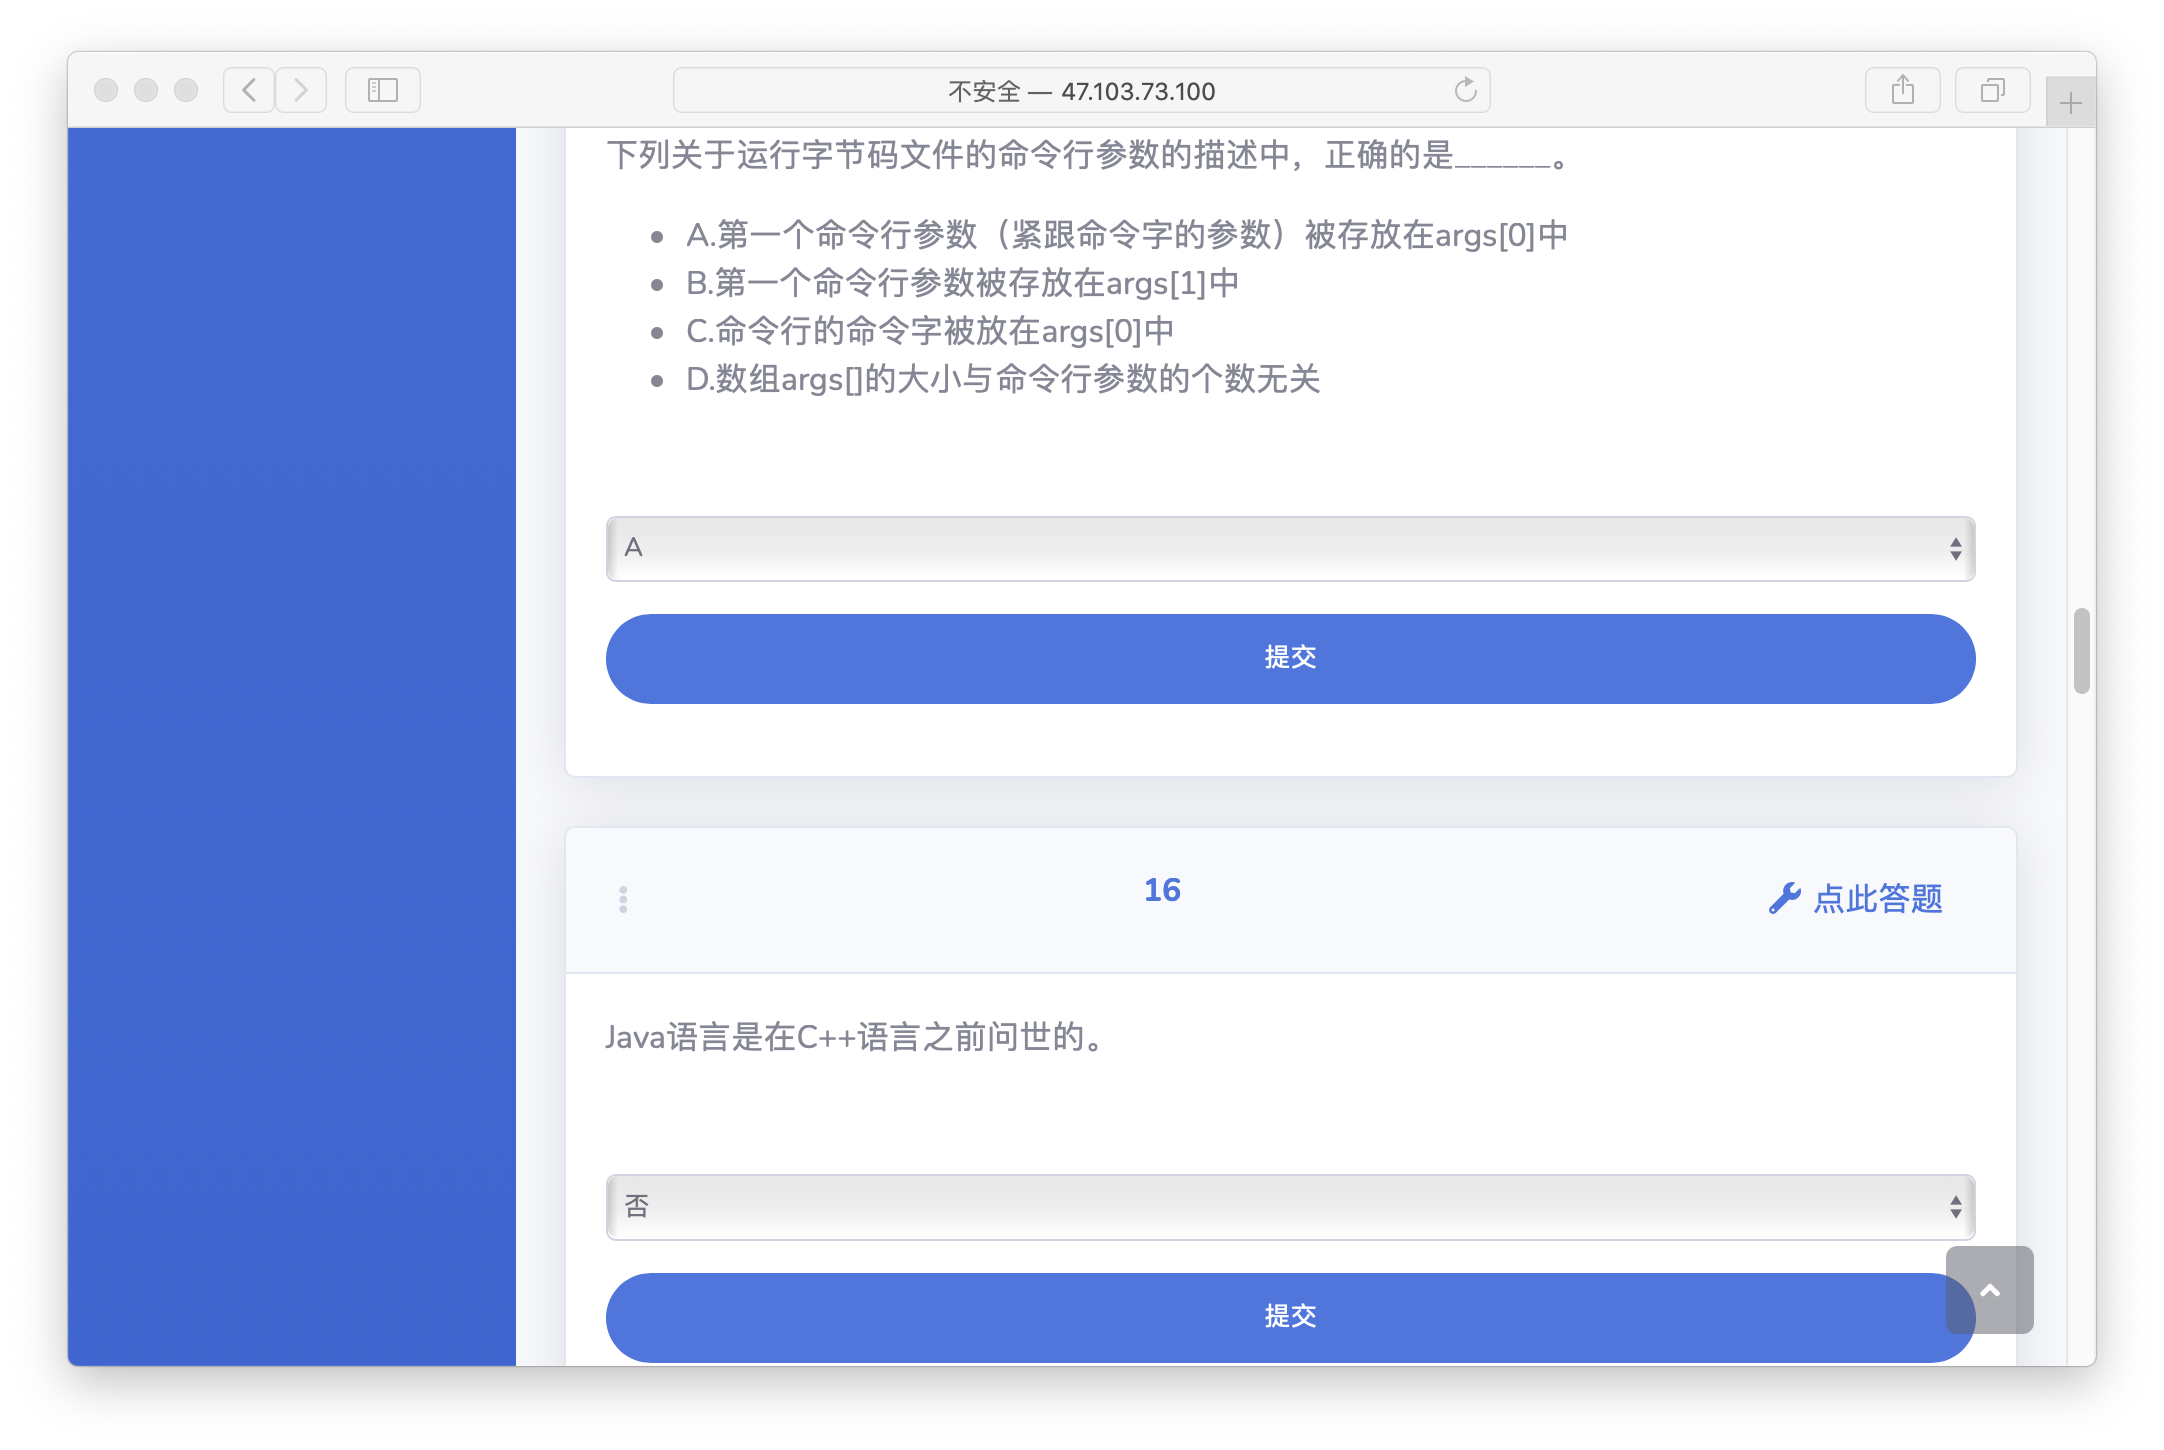
\includegraphics[width=0.8\textwidth]{answer_exercise.png}
  \caption{回答习题}
  \label{answer_exercise}
\end{figure}

\begin{figure}[htp]
  \centering
  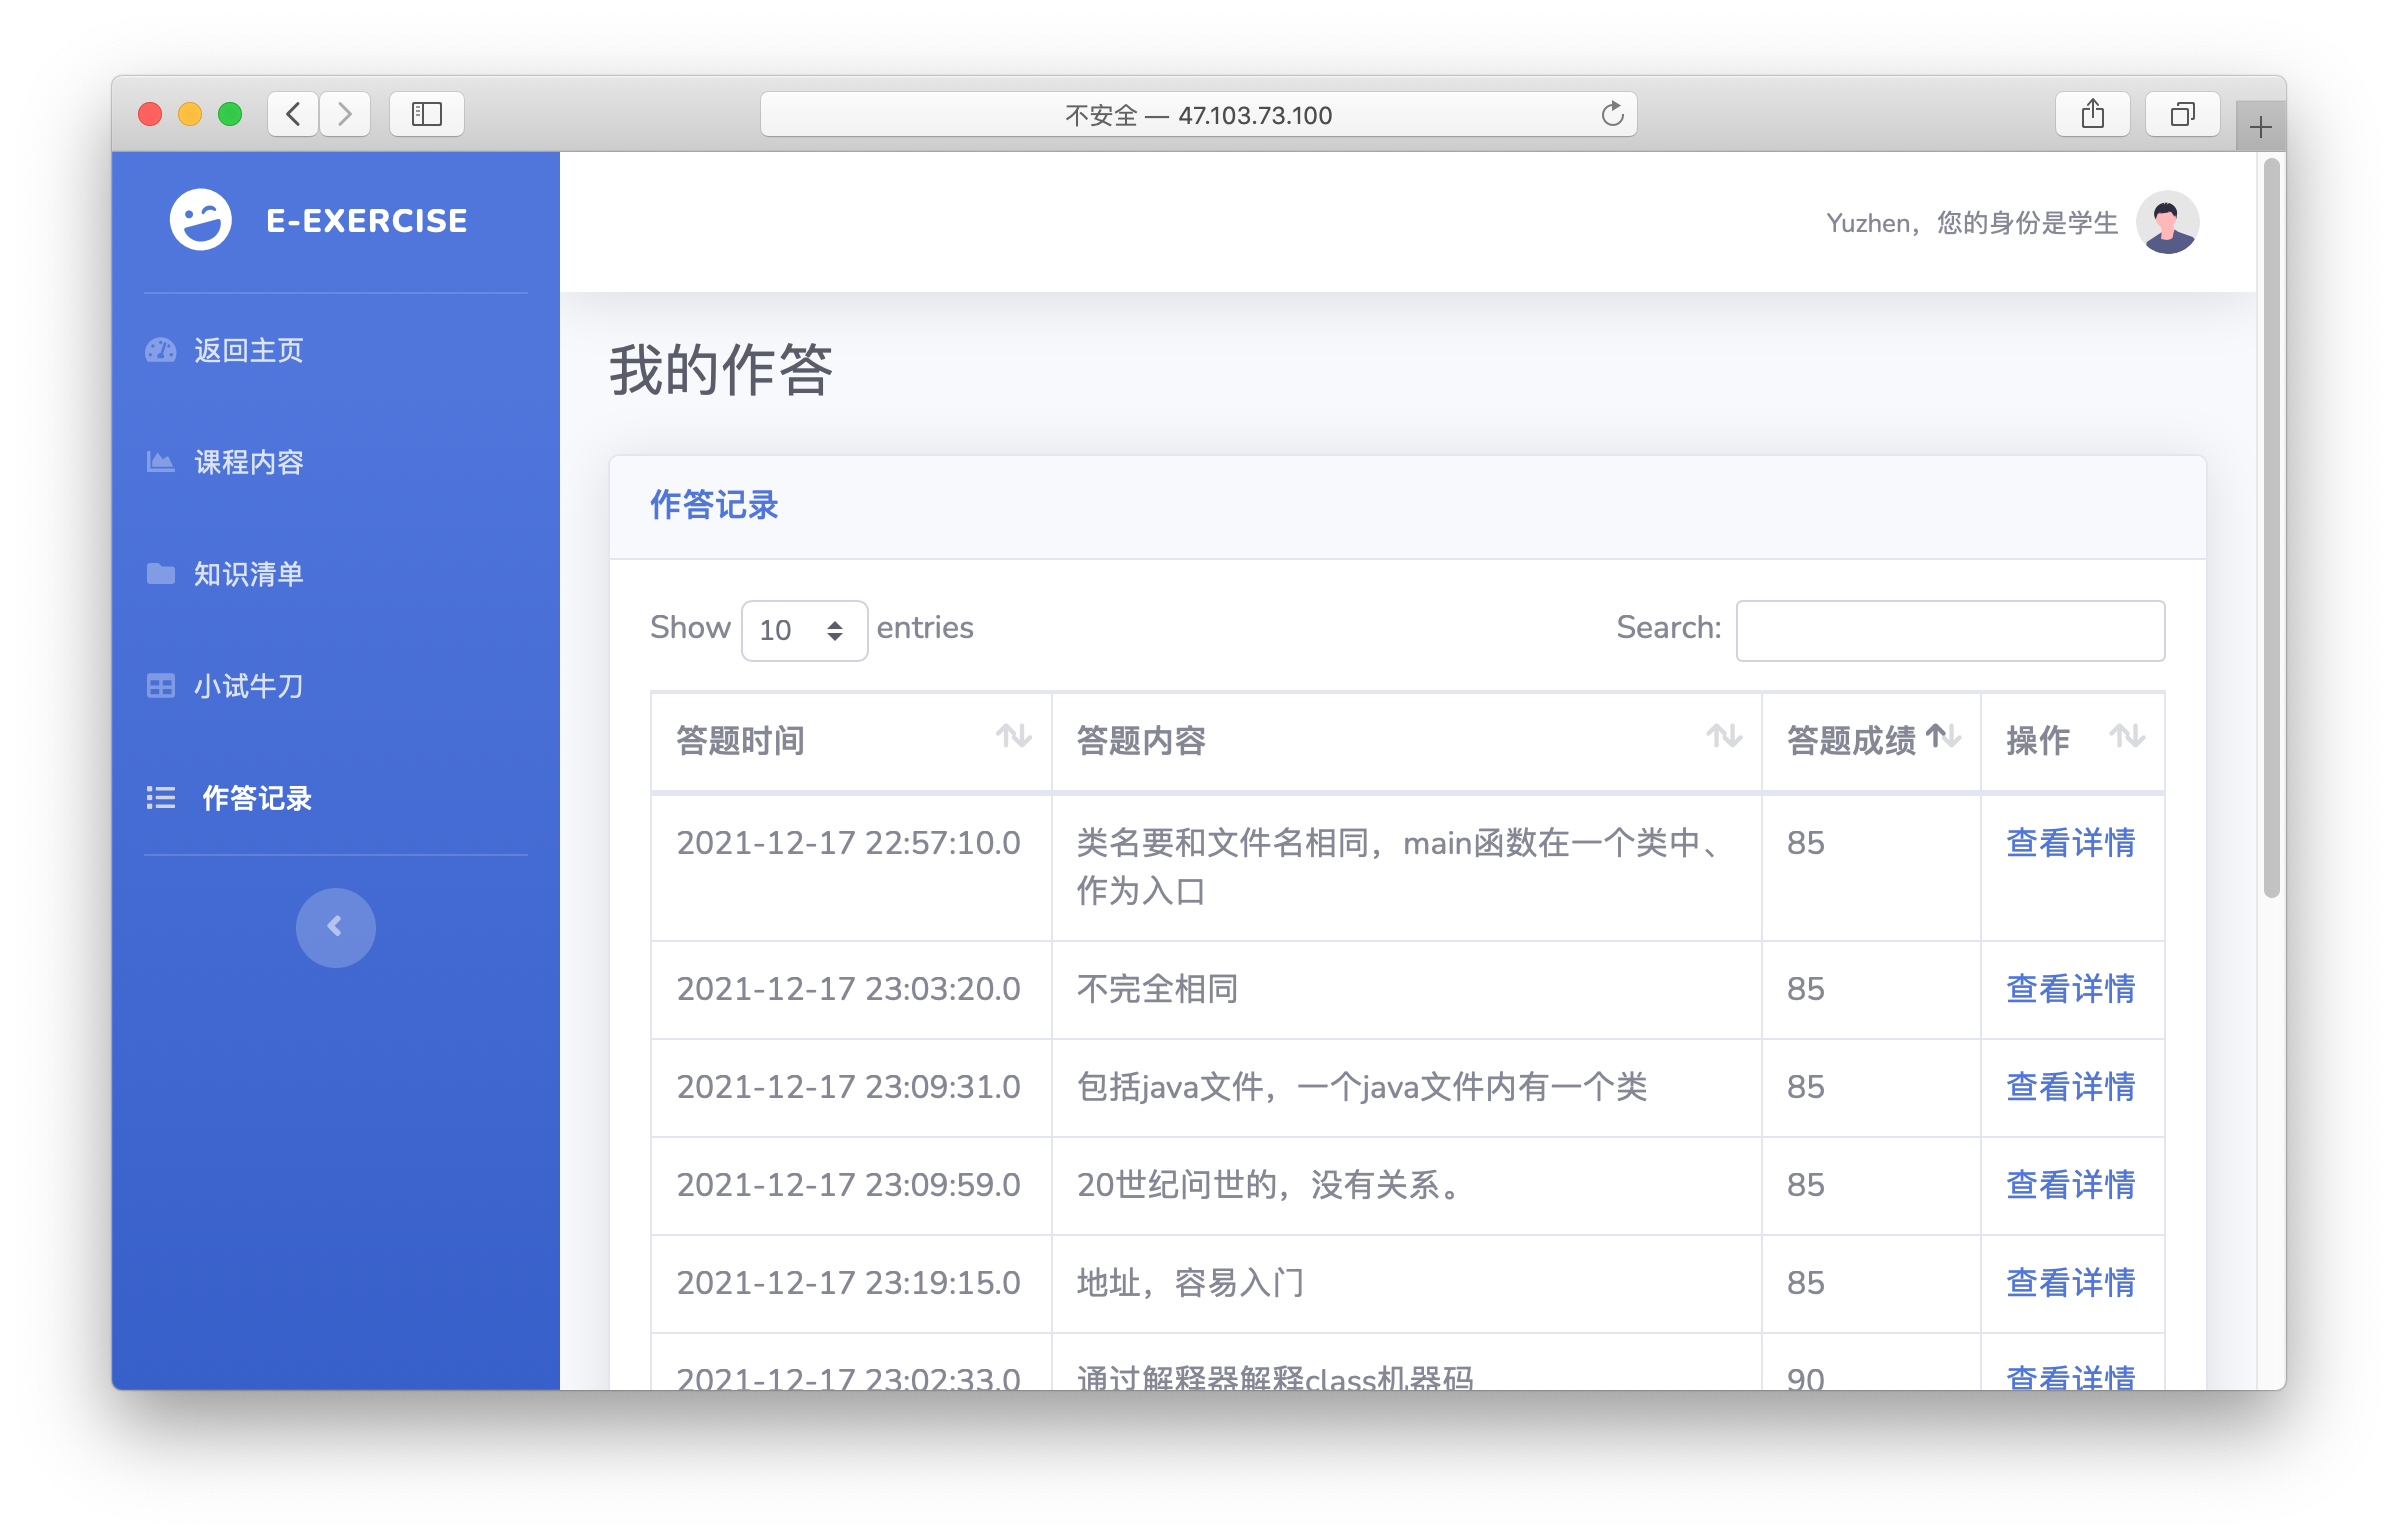
\includegraphics[width=0.8\textwidth]{answer_record.png}
  \caption{作答记录}
  \label{answer_record}
\end{figure}

\begin{figure}[htp]
  \centering
  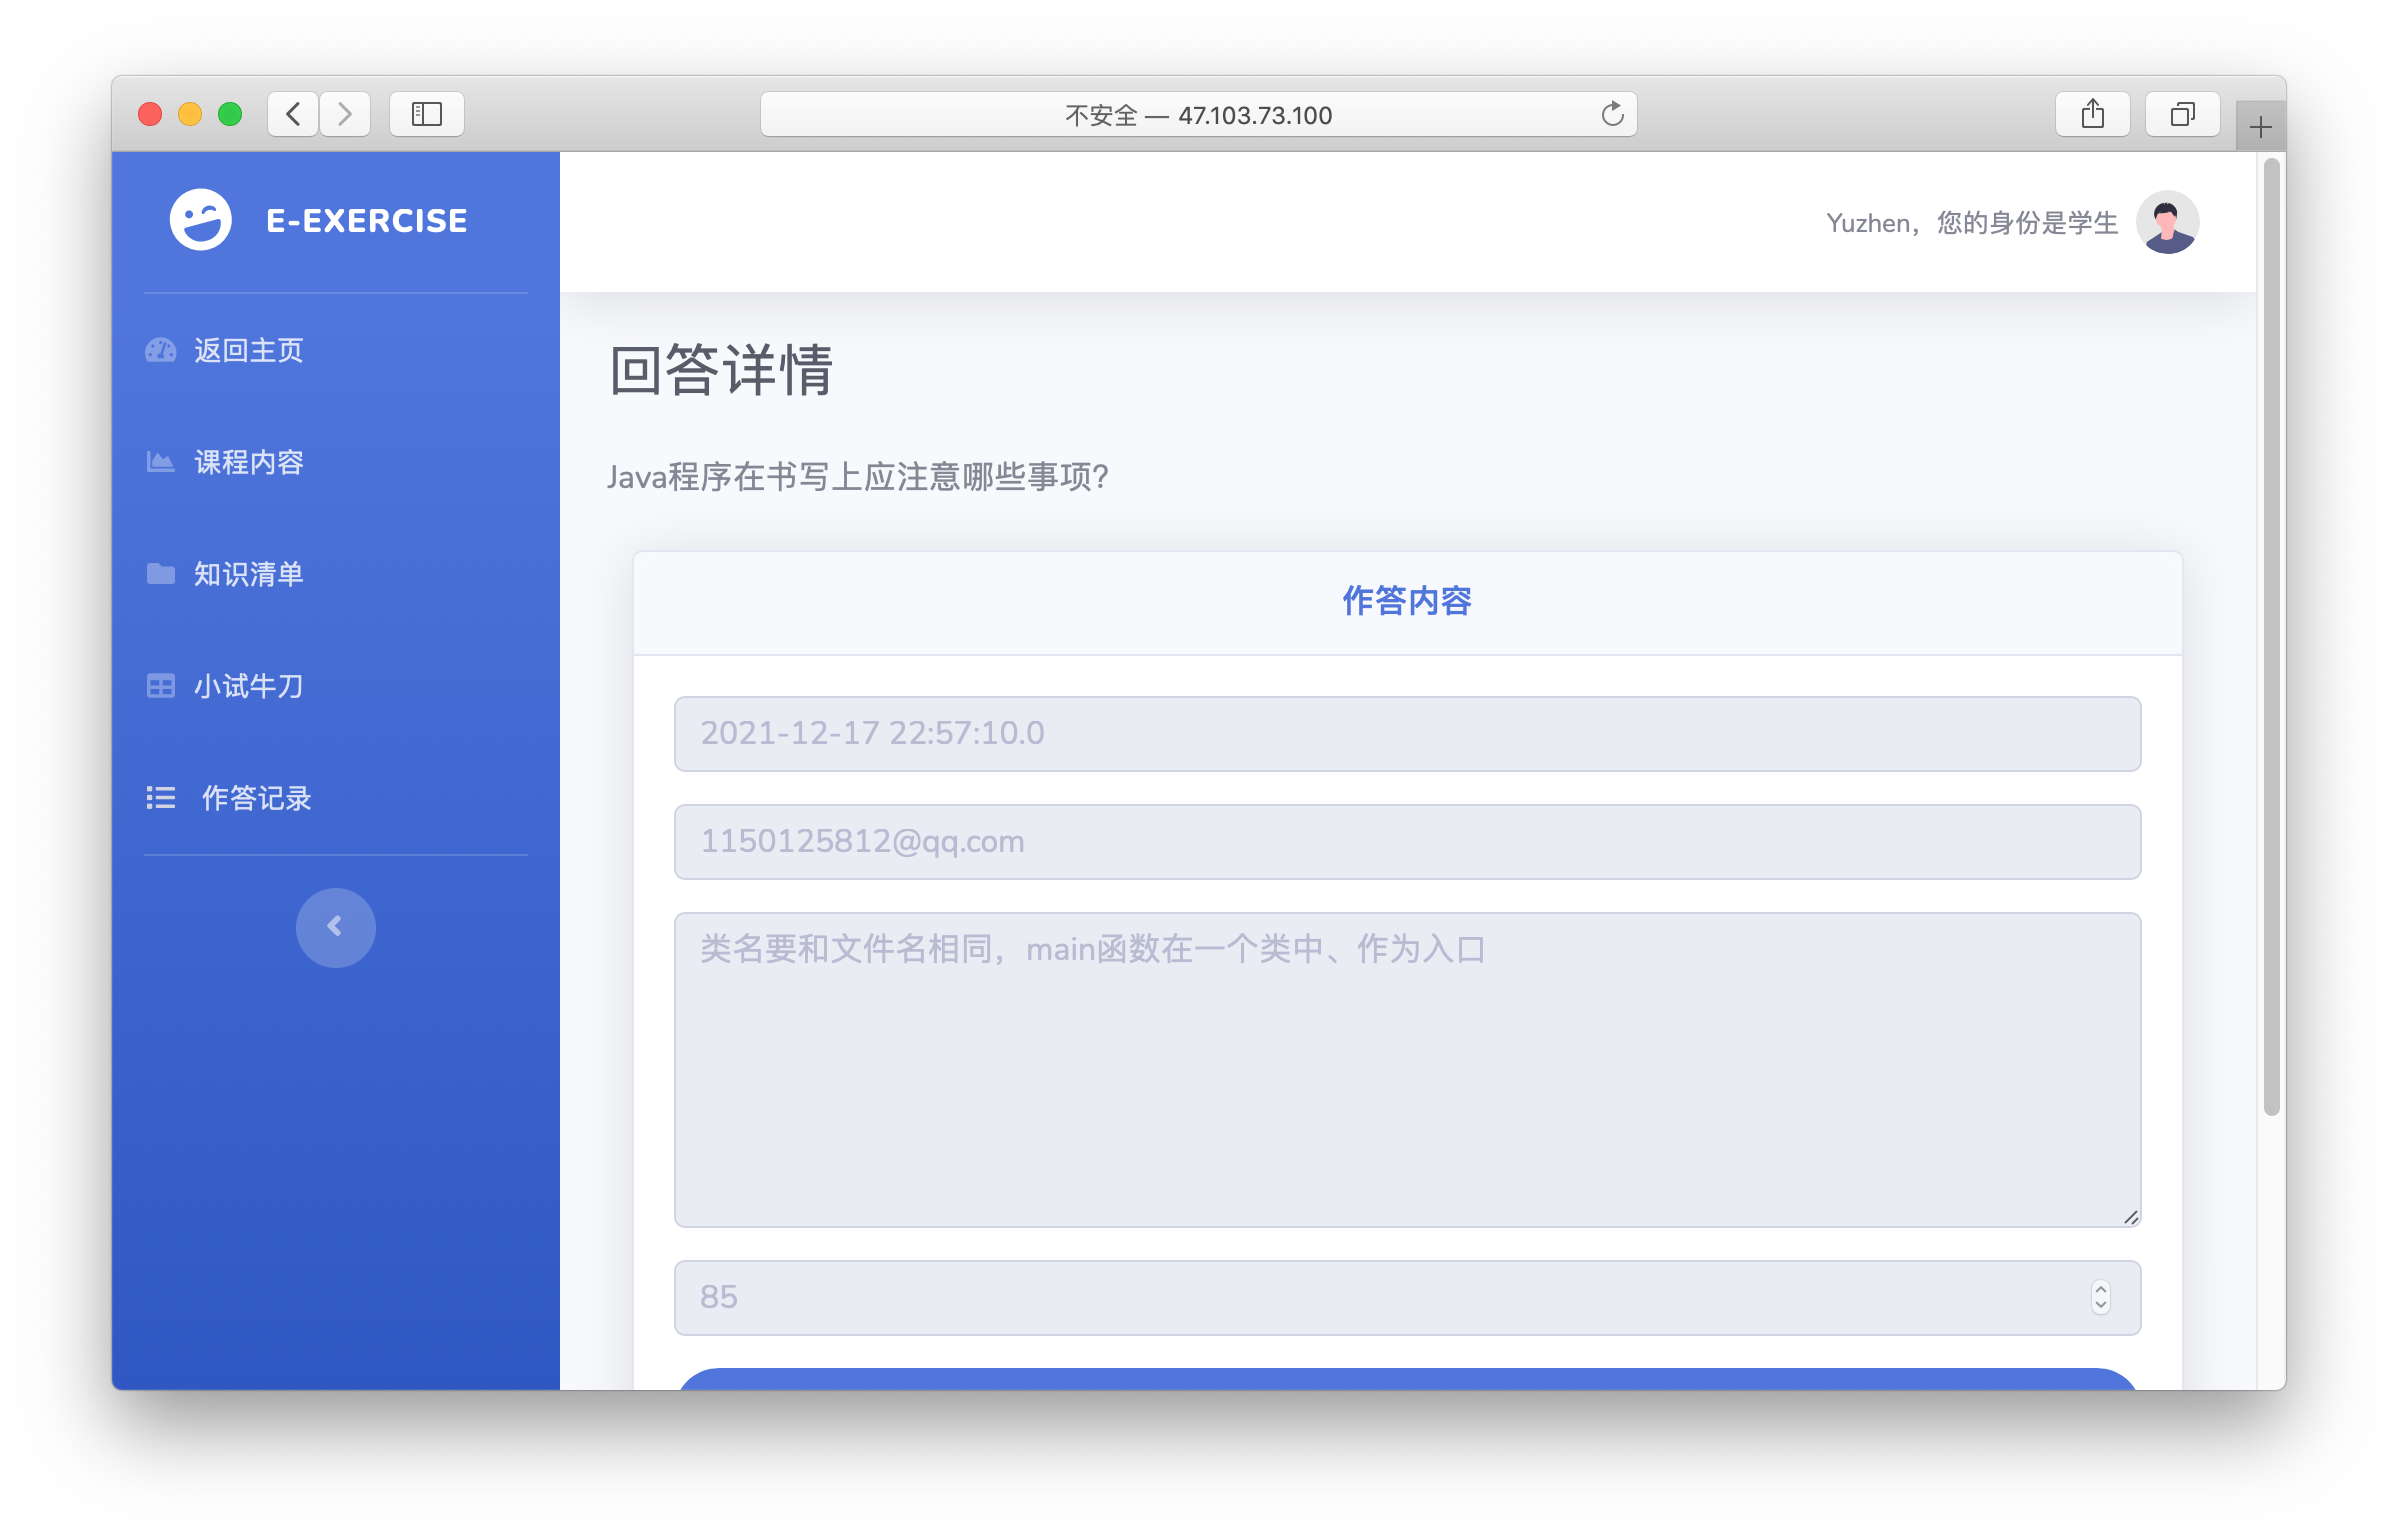
\includegraphics[width=0.8\textwidth]{answer_detail.png}
  \caption{作答详情}
  \label{answer_detail}
\end{figure}

学生可以在该页面进行答题,对于简答题,提供文本框;而对于选择题和判断题,提供选择框进行选择。如图\ref{recommend_exercise}和\ref{answer_exercise}所示。对于选择题和判断题,若添加习题时输入了答案,则系统会自行批改;其他情况交由教师批改。学生可在作答记录中查看自己的作答情况,如图\ref{answer_record}和\ref{answer_detail}所示。

对于管理员与教师来说,可以添加习题、修改习题、批改习题。添加习题、修改习题的界面与添加、修改知识的界面大致相同,批改习题的界面与学生查看答题详情的页面(如图\ref{answer_detail})类似,不同的是教师可以对成绩进行录入或修改。

习题内容也采用Markdown标记语言作为模板,在此基础上,还为选择题增添了标签。模板中用\verb|<opt>|标记选择题的选项,例如,图\ref{answer_exercise}中的选择题内容如下:
\begin{lstlisting}
  下列关于运行字节码文件的命令行参数的描述中,正确的是______。
  <opt>A.第一个命令行参数(紧跟命令字的参数)被存放在args[0]中
  <opt>B.第一个命令行参数被存放在args[1]中
  <opt>C.命令行的命令字被放在args[0]中
  <opt>D.数组args[]的大小与命令行参数的个数无关
\end{lstlisting}
此时,若有超过4个选项的习题,系统也能自动识别。

\newpage

\subsection{功能总览}

本网站的所有主体功能如图\ref{功能总览图}所示。

\begin{figure}[htp]
  \centering
  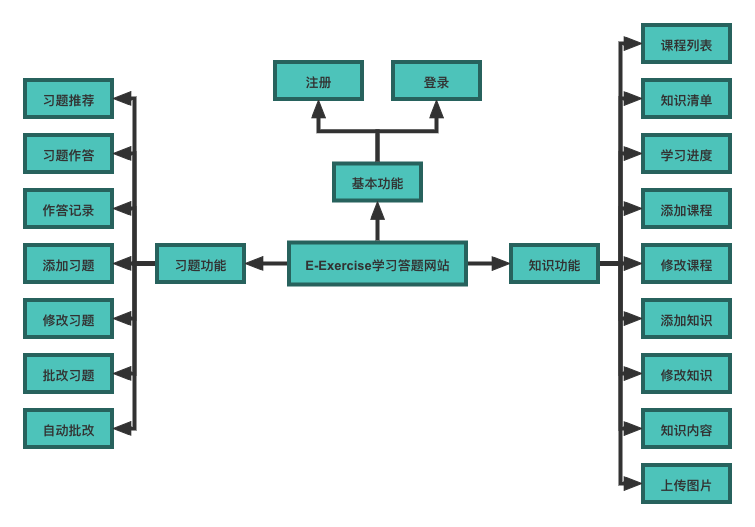
\includegraphics[width=0.8\textwidth]{功能总览图.png}
  \caption{功能总览}
  \label{功能总览图}
\end{figure}

% 打印参考文献表
% \printbibliography[heading=bibliography,title=参考资料]
\end{document}
